% Mini research note for the reduced-basis continuation lane.
\documentclass[11pt]{article}
% Shared preamble for the research-note series.
% Create note-specific content in the per-note directory; keep common macros here.
\usepackage[margin=1in]{geometry}
\usepackage[T1]{fontenc}
\usepackage[utf8]{inputenc}
\usepackage{amsmath,amssymb}
\usepackage{booktabs,longtable,array}
\usepackage{graphicx}
\usepackage{float}
\usepackage{enumitem}
\usepackage{xcolor}
\usepackage{hyperref}
\usepackage{caption}
\usepackage{titlesec}
\hypersetup{colorlinks=true, linkcolor=blue!60!black, urlcolor=blue!60!black, citecolor=blue!60!black}
\setlist[itemize]{leftmargin=1.25em, itemsep=0.2em, topsep=0.3em}
\setlist[enumerate]{leftmargin=1.4em, itemsep=0.2em, topsep=0.3em}
\setlength{\parindent}{0pt}
\setlength{\parskip}{0.6em}
\newcommand{\statusbox}[2]{%
  \noindent\fcolorbox{black}{gray!10}{%
    \parbox{\dimexpr\linewidth-2\fboxsep-2\fboxrule\relax}{%
      \textbf{Status:} #1\\#2
    }%
  }
}

% Shared notation helpers for the research-note series.
\newcommand{\Jlin}{J}
\newcommand{\Jphys}{J_{\mathrm{phys}}}
\newcommand{\Jsurf}{J_{\mathrm{surf}}}
\newcommand{\JdB}{J_{\mathrm{dB}}}
\newcommand{\phiopt}{\phi_{\mathrm{opt}}}
\newcommand{\sigmathreedb}{\sigma_{3\mathrm{dB}}}
\newcommand{\Nt}{N_t}
\newcommand{\Nphi}{N_{\phi}}
\newcommand{\Lfiber}{L}
\newcommand{\Pcont}{P}
\newcommand{\band}{\mathcal{B}_{\mathrm{Raman}}}
\newcommand{\todoitem}[1]{\textcolor{red!70!black}{\textbf{TODO:} #1}}


\title{Reduced-Basis Continuation for Raman Suppression}
\author{Fiber Raman Suppression Project}
\date{Evidence snapshot: 2026-04-28}

\begin{document}
\maketitle

\begin{abstract}
Reduced-basis continuation is the clearest basin-access result in the
single-mode Raman-suppression program. On the canonical SMF-28 test case,
continuation through a local cubic-spline phase basis reaches about
\(-67.6\,\mathrm{dB}\), while full-grid L-BFGS from zero phase stalls near
\(-57.8\,\mathrm{dB}\) under the same physical objective. The unrestricted
search space has more degrees of freedom, but the structured continuation path
finds a deeper basin. A later full-grid refinement check shows that the result
is not merely a reduced-coordinate artifact: reduced-basis seeds carry into
strong full-grid solutions. The limitation is equally important: the deepest
solutions are narrow and fiber-specific, while the most transferable profiles
are much shallower.
\end{abstract}

\section*{Claim Status}
\statusbox{strong simulated result; portability and rerun packaging still open}{The
basin-access claim is supported by the basis sweep, full-grid penalty sweep,
transfer tests, robustness tests, and continuation-seeded full-grid refinements.
The result should be treated as a strong simulated finding, not a finished
hardware recipe. What remains unresolved is how to preserve its depth while
improving robustness, transferability, and one-command reproducibility.}

\section{Question and Thesis}

The question is simple: is a low-dimensional spectral-phase basis only a way to
make the problem smaller, or does it actually help the optimizer find a better
solution?

The evidence supports the stronger interpretation. A sequence of structured
reduced problems guides L-BFGS into a deeper solution family than direct
zero-start optimization on the full spectral grid. This is counterintuitive but
central: the full-grid problem has more control freedom, yet the zero-start
trajectory consistently lands in a shallower basin.

The result should not be read as ``cubic splines are the true physics.'' It
should be read as an optimizer-path result:
\[
    \text{structured path} \;+\; \text{local phase support}
    \quad \Longrightarrow \quad
    \text{better basin access}.
\]

\section{Setup and Objective}

The canonical benchmark is a phase-only input shaping problem for SMF-28 at
\[
    L = 2\,\mathrm{m}, \qquad P = 0.2\,\mathrm{W}, \qquad \Nt = 16384 .
\]
The input field is represented on a frequency grid. A trial spectral phase
\(\phi(\omega)\) changes only the phase of the pulse, not its spectral
amplitude:
\[
    u_\omega(0;\phi) = u_{\omega,0}\exp(i\phi).
\]
That shaped field is propagated through the interaction-picture GNLSE solver to
obtain \(u_\omega(L;\phi)\). The physical Raman objective is the fraction of
output spectral energy inside the Raman-shifted band \(\band\):
\[
    E_{\band}(\phi) =
    \sum_{\omega_k\in\band} |u_{\omega_k}(L;\phi)|^2\,\Delta\omega,
    \qquad
    E_{\mathrm{tot}}(\phi) =
    \sum_k |u_{\omega_k}(L;\phi)|^2\,\Delta\omega,
\]
\[
    \Jphys(\phi) =
    \frac{E_{\band}(\phi)}{E_{\mathrm{tot}}(\phi)}.
\]
Lower is better. In plots and tables the same quantity is reported in decibels,
\[
    \JdB(\phi)=10\log_{10}\Jphys(\phi).
\]

The actual optimizer can use a regularized scalar surface. In the maintained
code path, regularizers are added on the linear surface first:
\[
    \Jsurf(\phi)
    =
    \Jphys(\phi)
    + \lambda_{\mathrm{gdd}} R_{\mathrm{gdd}}(\phi)
    + \lambda_{\mathrm{edge}} R_{\mathrm{edge}}(\phi).
\]
Here \(R_{\mathrm{gdd}}\) penalizes large second differences of phase on the
frequency grid, while \(R_{\mathrm{edge}}\) penalizes shaped input pulses that
place too much temporal energy at the FFT-window edges. The GDD term is
implemented as
\[
    R_{\mathrm{gdd}}(\phi)
    =
    \sum_{i=2}^{\Nt-1}
    \frac{\left(\phi_{i+1}-2\phi_i+\phi_{i-1}\right)^2}{\Delta\omega^3},
\]
with the coefficient \(\lambda_{\mathrm{gdd}}\) applied outside the sum. The
edge term is an input-window energy fraction after applying the phase. The
default reduced-basis sweep used the unregularized physics objective
\((\lambda_{\mathrm{gdd}}=\lambda_{\mathrm{edge}}=0)\); the separate full-grid
penalty sweep tested whether these regularizers could recover the same basin.

When \(\texttt{log\_cost=true}\), L-BFGS sees the log surface
\[
    F(\phi) = 10\log_{10}\Jsurf(\phi).
\]
The gradient is scaled by the matching chain rule,
\[
    \nabla_\phi F
    =
    \frac{10}{\ln 10}
    \frac{1}{\Jsurf(\phi)}
    \nabla_\phi \Jsurf,
\]
so the scalar objective and the gradient given to L-BFGS are on the same scale.
This matters at deep suppression, where the linear Raman fraction is tiny and
an unscaled gradient can become numerically unhelpful.

The fiber model and propagation numerics follow standard nonlinear fiber-optics
and interaction-picture split-step/RK practice
\cite{agrawal2019,dudley2006,hult2007}. The project gradient is computed by an
adjoint solve: one forward propagation gives the output field and one backward
adjoint propagation gives \(\nabla_\phi F\). This avoids finite-differencing
thousands of phase pixels.

\subsection*{Full Derivative Chain}

The complete computational chain for one reduced-basis trial is
\[
    c
    \xrightarrow{\;\phi = Bc\;}
    u_\omega(0;c)=u_{\omega,0}\exp(iBc)
    \xrightarrow{\;\mathrm{GNLSE}\;}
    u_\omega(L;c)
    \xrightarrow{\;\mathrm{Raman\;band\;fraction}\;}
    F(c).
\]
For the physical output objective \(J=E_{\band}/E_{\mathrm{tot}}\), the
terminal sensitivity with respect to an output spectral sample \(U_k\) is
\[
    \frac{\partial J}{\partial U_k^\ast}
    =
    \frac{\chi_k-J}{E_{\mathrm{tot}}}U_k,
\]
where \(\chi_k=1\) inside the Raman band and \(\chi_k=0\) outside it. The
adjoint propagation pulls this output sensitivity back to the input spectrum.
If the input spectral sensitivity is \(g_{u_0}\), then a phase perturbation
\(\delta\phi\) gives
\[
    \delta u_{\omega,k}(0)= i u_{\omega,k}(0)\,\delta\phi_k,
    \qquad
    \delta F
    =
    \nabla_\phi F^\top \delta\phi .
\]
The reduced basis then adds only one more chain-rule step:
\[
    \delta\phi = B\,\delta c,
    \qquad
    \delta F
    =
    \nabla_\phi F^\top B\,\delta c
    =
    \left(B^\top\nabla_\phi F\right)^\top\delta c.
\]
That is the reason the coefficient gradient is \(B^\top\nabla_\phi F\).
Nothing about the fiber solver is reduced; only the input-control coordinates
are reduced.

\subsection*{Intuition Check}

The cost function asks a simple question: after the pulse leaves the fiber, what
fraction of its energy landed in the Raman band? The optimizer tries to make
that fraction small by changing only the input spectral phase. The log scale
does not change which physical result is better; it makes very small Raman
fractions easier for L-BFGS to optimize.

\subsection*{TL;DR}

The math chain is: choose coefficients \(c\), build a full phase mask
\(\phi=Bc\), propagate the full-resolution pulse, measure Raman energy, then
send the adjoint gradient back through the same chain. The forward map uses
\(B\); the backward gradient map uses \(B^\top\).

\section{Reduced-Basis Method}

The easiest way to think about the reduced basis is as a subspace of allowed
phase profiles. The full problem has \(\Nt=16384\) phase pixels, so a completely
free optimizer can move in \(16384\) independent directions. A reduced-basis
run picks only \(\Nphi\) allowed directions first, then asks the optimizer to
choose how much of each direction to use.

The reduced problem writes the full-grid phase as
\[
    \phi = Bc, \qquad
    B\in\mathbb{R}^{\Nt\times\Nphi}, \qquad
    c \in \mathbb{R}^{\Nphi}, \qquad
    \Nphi \ll \Nt ,
\]
where \(B\) is a basis or interpolation operator. This is the central
constraint: L-BFGS is never allowed to choose an arbitrary \(\Nt\)-pixel phase
while it is in a reduced run. It only chooses \(c\). Every trial phase is built
as \(Bc\), passed to the same full-resolution forward solver, and then
discarded after the cost and gradient are evaluated.

\begin{figure}[H]
\centering
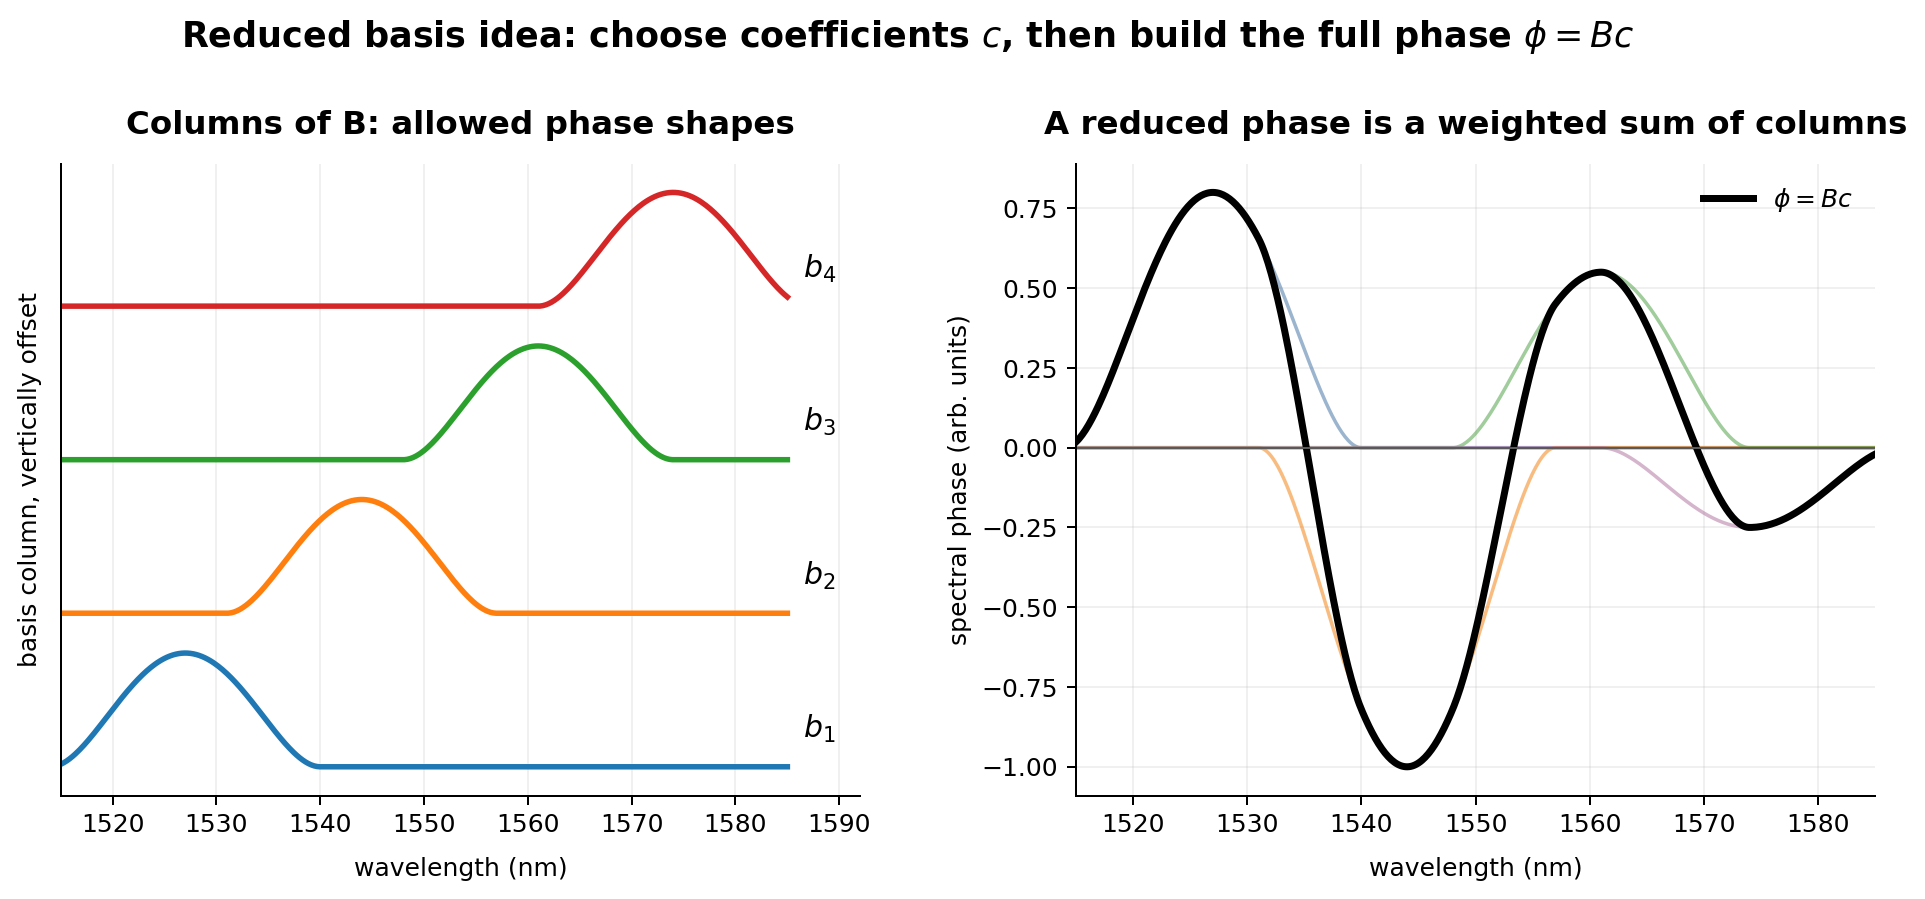
\includegraphics[width=0.92\linewidth]{figures/basis_linear_algebra_diagram.png}
\caption{Linear-algebra picture of the reduced basis. Each column of \(B\) is
one allowed full-grid phase shape. The coefficient vector \(c\) says how much
of each column to mix in. The product \(Bc\) is still a full-resolution phase
vector; it just lives in a lower-dimensional subspace.}
\end{figure}

For a small example, imagine \(\Nt=5\) grid points but only two allowed shapes:
\[
    B =
    \begin{bmatrix}
    1 & 0\\
    0.7 & 0.2\\
    0.2 & 1\\
    0 & 0.7\\
    0 & 0.1
    \end{bmatrix},
    \qquad
    c =
    \begin{bmatrix}
    c_1\\ c_2
    \end{bmatrix},
    \qquad
    \phi =
    \begin{bmatrix}
    1c_1\\
    0.7c_1+0.2c_2\\
    0.2c_1+1c_2\\
    0.7c_2\\
    0.1c_2
    \end{bmatrix}.
\]
The optimizer can change \(c_1\) and \(c_2\), but it cannot set the five
entries of \(\phi\) independently. That restriction is the point: it forces the
phase to be a smooth combination of a few meaningful shapes instead of a
pixel-by-pixel pattern.

The coefficient problem is
\[
    \min_c \; F(Bc).
\]
For any coefficient \(c_j\),
\[
    \frac{\partial F(Bc)}{\partial c_j}
    =
    \sum_{i=1}^{\Nt}
    \frac{\partial F}{\partial \phi_i}
    \frac{\partial \phi_i}{\partial c_j}
    =
    \sum_{i=1}^{\Nt}
    \frac{\partial F}{\partial \phi_i} B_{ij}.
\]
Therefore the reduced gradient is
\[
    \nabla_c F(Bc) = B^\top \nabla_\phi F(\phi).
\]
This is not a heuristic projection after the fact. It is the exact adjoint of
the linear map \(c\mapsto Bc\). If the full adjoint gradient says changing
\(\phi_i\) would help, the reduced gradient only keeps the part of that
information that can be produced by changing the allowed coefficients.

\subsection*{How The Cubic Basis Is Built}

For the cubic-spline runs, the code first marks the pulse bandwidth: bins where
the input spectral power is more than \(1\%\) of its peak. It then works on the
\(\texttt{fftshift}\)-ordered frequency axis so that this bandwidth is a
contiguous block. The \(\Nphi\) coefficients are knot values spread evenly over
that block. Each column of \(B\) is the full-grid phase produced by setting one
knot to one and the other knots to zero, then cubic-spline interpolating across
the bandwidth. Rows outside the pulse bandwidth are zeroed.

In plain terms, a coefficient means ``move this local smooth phase knot,'' not
``move one arbitrary FFT pixel.'' The optimizer still receives an exact
gradient, but only for the smooth phase shapes that the basis can represent.
The full-grid solver is unchanged; only the control parameterization is
restricted.

\subsection*{Intuition Check}

The short version of the reduced-basis idea is:

\begin{quote}
The original optimization has one knob for every frequency pixel. The
reduced-basis run replaces those thousands of knobs with a smaller set of
smooth phase-shape knobs. Mathematically, I store those allowed shapes as the
columns of a matrix \(B\). The optimizer chooses coefficients \(c\), and the
actual phase sent into the simulation is \(Bc\). So the simulation is still
full resolution, but the optimizer is only allowed to move inside the subspace
spanned by the columns of \(B\).
\end{quote}

The gradient follows the same idea. The adjoint solve first tells us how the
cost would change if each full-grid phase pixel moved. Multiplying by
\(B^\top\) converts that full-grid information into answers for the smaller
question: ``how should each coefficient move?''

\subsection*{Verification Cross-Check}

This note uses the same reduced-coordinate equation derived in the independent
verification pass:
\[
    d\phi = B\,dc,
    \qquad
    dF = \nabla_\phi F^\top d\phi
        = \nabla_\phi F^\top B\,dc
        = (B^\top\nabla_\phi F)^\top dc.
\]
So the coefficient-space gradient is
\[
    \boxed{\nabla_c F = B^\top \nabla_\phi F.}
\]
This formula does not require \(B\) to have orthonormal columns. If the columns
are not orthonormal, \(B^\top\nabla_\phi F\) is still the correct gradient in
the optimizer coordinates \(c\). A pseudoinverse or Gram matrix only appears if
we ask a different question: ``what is the closest full-grid projection of a
vector onto the span of \(B\)?''

The practical verification test is finite-difference in coefficient space:
\[
    \frac{F(B(c+h v))-F(B(c-h v))}{2h}
    \approx
    (B^\top\nabla_\phi F)^\top v .
\]
This matters because checking the full-grid phase gradient alone is not enough.
The reduced run must also prove that the gradient was chained back to the
actual coordinates seen by L-BFGS.

\subsection*{TL;DR}

The clean explanation is: \(B\) turns a short coefficient vector into a full
phase mask, and \(B^\top\) turns the full adjoint gradient back into
coefficient gradients. \(B\) sends controls into the simulator; \(B^\top\)
sends sensitivities back to the optimizer.

\subsection*{Continuation}

Continuation changes the initial condition rather than only the coordinate
system. If \(B_k\) and \(B_{k+1}\) are consecutive bases in a ladder, the next
seed is obtained by lifting the previous optimum:
\[
    c_{k+1}^{(0)}
    \approx \arg\min_c \left\| B_{k+1}c - B_k c_k^\star \right\|_2^2 .
\]
The optimizer therefore does not restart from \(\phi \equiv 0\). It walks
through a sequence of smoother nearby problems before entering the high
dimensional search space. This is the same basic idea behind continuation
methods: solve an easier nearby problem first, then use that solution to start
the harder problem \cite{allgower1990}.

The full-grid refinement check is the only step that deliberately removes the
reduced-basis restriction. There, the optimized phase \(Bc^\star\) is used as
the initial full-grid phase, and L-BFGS is then allowed to move all \(\Nt\)
phase pixels. That is why the refinement test is a strong sanity check: if the
reduced solution were only good because the basis hid important descent
directions, unrestricted refinement would immediately expose that.

\subsection*{Intuition Check}

Continuation is not just ``use fewer knobs.'' It is ``walk to the hard problem
through easier versions of the problem.'' The early low-dimensional runs find a
reasonable phase family without letting the optimizer chase every pixel. Later
runs add more freedom after the optimizer is already near a useful basin.

\section{Experimental Strategy}

The evidence comes from four linked tests. They answer different questions, so
they should not be collapsed into one headline number.

\begin{enumerate}
    \item \textbf{Basis-family sweep.} Polynomial, chirp-ladder, DCT, linear,
    and cubic-spline parameterizations were optimized over increasing
    dimensions. This tests whether the result is special to one basis family or
    whether many simple parameterizations can find the same basin.
    \item \textbf{Full-grid penalty sweep.} The full spectral grid was optimized
    from zero phase with smoothness and sparsity penalties. This tests whether
    regularization alone can recover the continuation basin without changing
    the start path.
    \item \textbf{Robustness and transfer evaluation.} Each candidate was
    checked for local phase-noise basin width, neighboring physical settings,
    and direct transfer to an HNLF setting. The reported
    \(\sigmathreedb\) is the approximate random phase-noise size where
    performance degrades by \(3\,\mathrm{dB}\).
    \item \textbf{Full-grid refinement.} Reduced-basis optima were used as seeds
    for a final full-grid L-BFGS step to test whether the reduced solution
    survives outside its coordinate restriction.
\end{enumerate}

The experimental logic is:
\[
\begin{array}{c}
\text{choose basis family and dimension}\\
\downarrow\\
\text{construct }B\text{ on the pulse bandwidth}\\
\downarrow\\
\text{optimize }c\text{ with full-resolution propagation}\\
\downarrow\\
\text{save }\phi=Bc\text{ and standard diagnostics}\\
\downarrow\\
\text{compare depth, width, transfer, and full-grid refinement.}
\end{array}
\]

The main cubic continuation ladder uses increasingly flexible local spline
spaces. Lower-dimensional runs are smoother and easier for L-BFGS to navigate;
higher-dimensional runs can represent sharper phase structure once a useful
basin has already been reached. The comparison baselines are important:
zero-start full-grid L-BFGS tests direct high-dimensional optimization, and the
penalty sweep tests whether smoothness penalties alone can imitate
continuation.

\subsection*{Interpretive Summary}

The experiment is designed to separate three ideas that can otherwise get mixed
together: smaller search spaces, better optimization paths, and better final
solutions. The key finding is that the continuation path matters. A full-grid
optimizer has more freedom, but from zero phase it does not enter the same deep
basin that the reduced-basis path finds.

\section{Representative Results}

\begin{figure}[H]
\centering
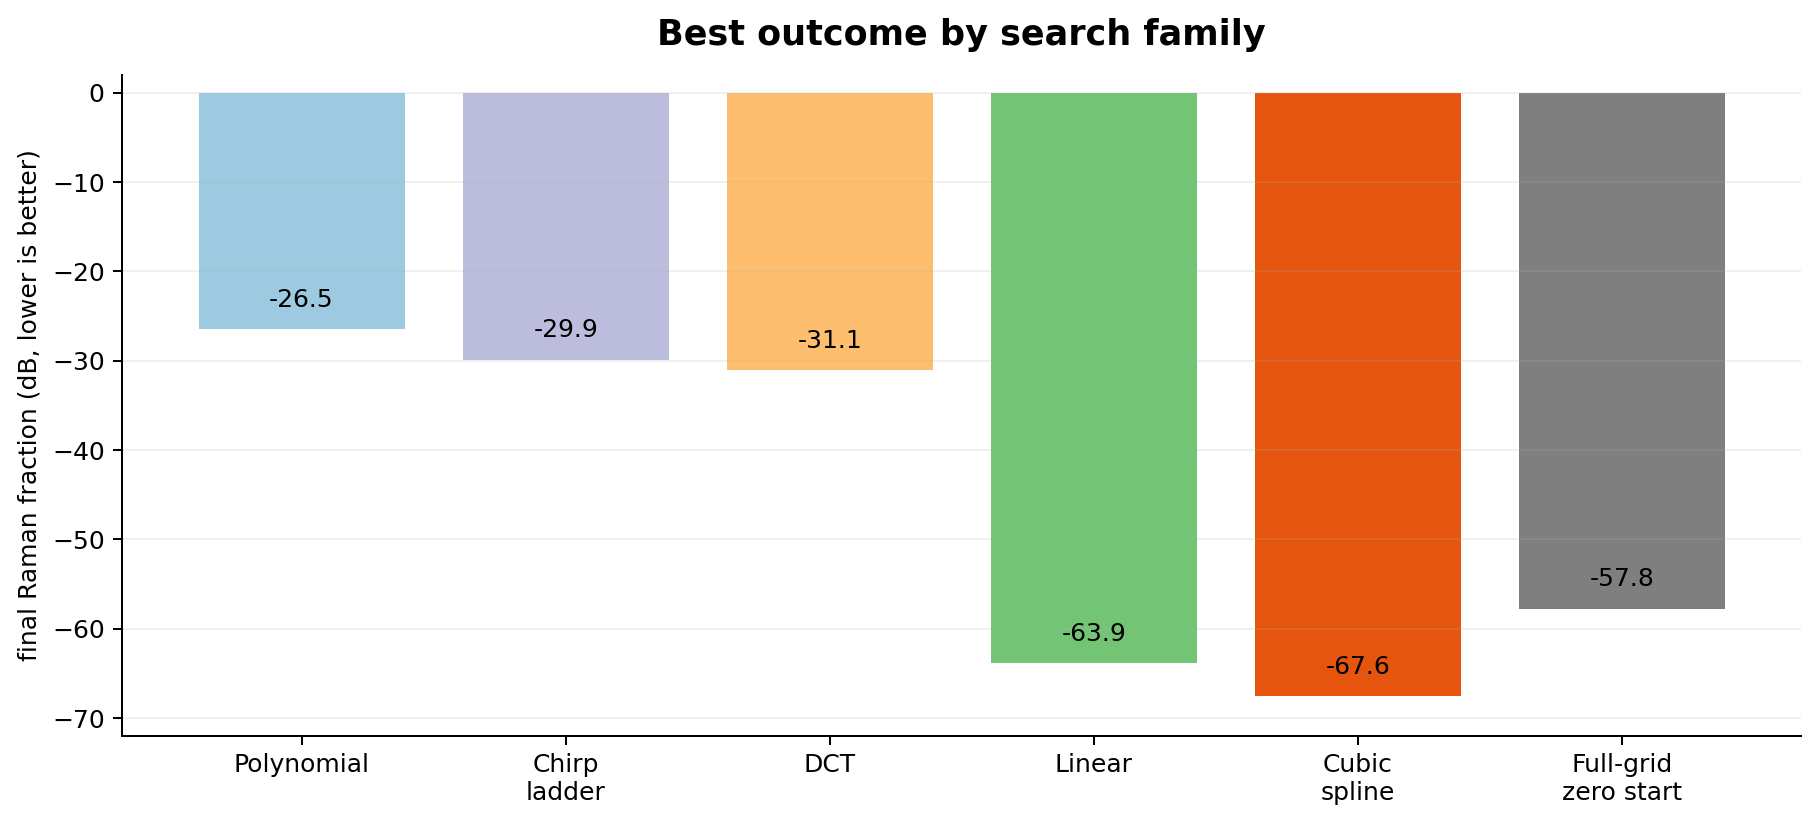
\includegraphics[width=0.92\linewidth]{figures/basis_family_depth_summary.png}
\caption{Best objective reached by each search family. Local cubic splines are
the deepest reduced-basis family, and the direct full-grid zero-start baseline
does not reach the same basin.}
\end{figure}

\begin{center}
\small
\begin{tabular}{l r r r l}
\toprule
Approach & Final \(\JdB\) & \(\sigmathreedb\) & HNLF gap & Main lesson \\
\midrule
Cubic spline, 128 coeffs. & -67.60 & 0.072 & +21.50 & Deepest canonical result \\
Cubic spline, 32 coeffs. & -60.77 & 0.143 & +16.50 & Better width, less depth \\
Linear basis, 64 coeffs. & -63.94 & 0.093 & +20.80 & Strong low-complexity path \\
Polynomial, 3 coeffs. & -26.50 & \(>1\) & +0.29 & Most transferable profile \\
Full grid, zero start & -57.75 & 0.17 & +15.6 & Shallower direct basin \\
\bottomrule
\end{tabular}
\captionof{table}{Representative outcomes from the reduced-basis, transfer,
and full-grid comparison runs. The table is deliberately limited to the rows
needed to explain the tradeoff; the full sweeps contain 41 candidates.}
\end{center}

\textbf{How to read the columns.} \(\JdB\) is the final Raman-band energy
fraction in decibels, so more negative is better. \(\sigmathreedb\) is the
approximate random phase-noise scale where the result becomes \(3\,\mathrm{dB}\)
worse; larger means a wider local basin. The HNLF gap is the loss in
suppression when the same phase is evaluated on a different high-nonlinearity
fiber setting; smaller gap means better transfer.

\begin{figure}[H]
\centering
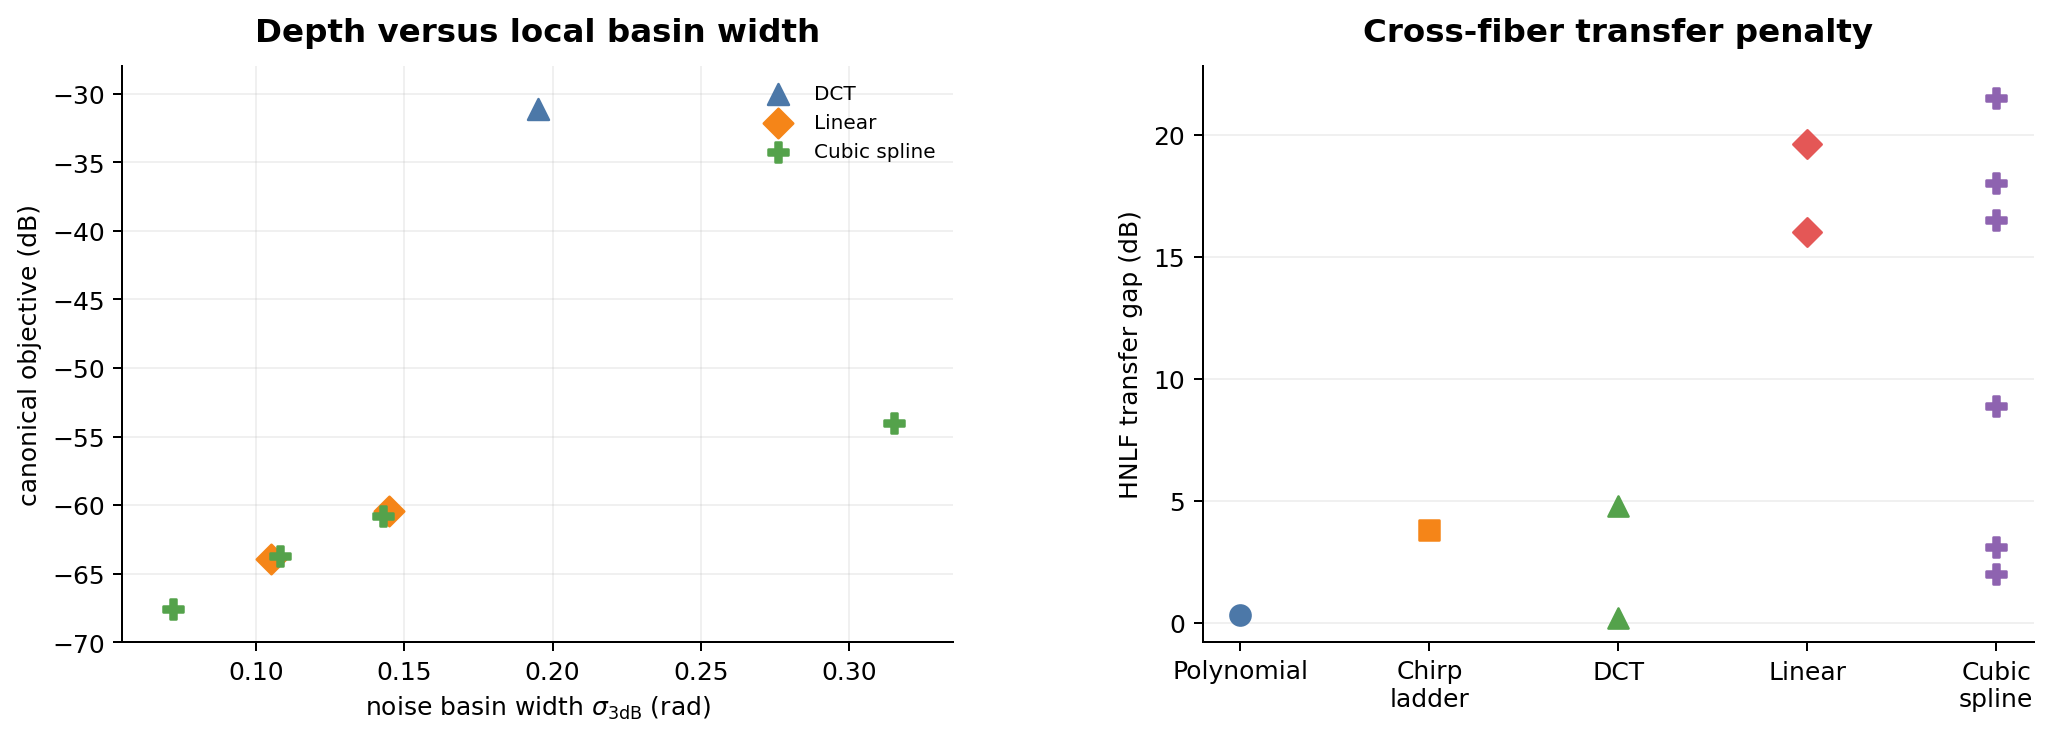
\includegraphics[width=0.92\linewidth]{figures/robustness_transfer_tradeoff.png}
\caption{Reduced-basis candidates separate into different regimes. The deepest
cubic solutions have narrow phase-noise basins and poor HNLF transfer; the
simple polynomial profile is much shallower but transfers almost unchanged.}
\end{figure}

\begin{figure}[H]
\centering
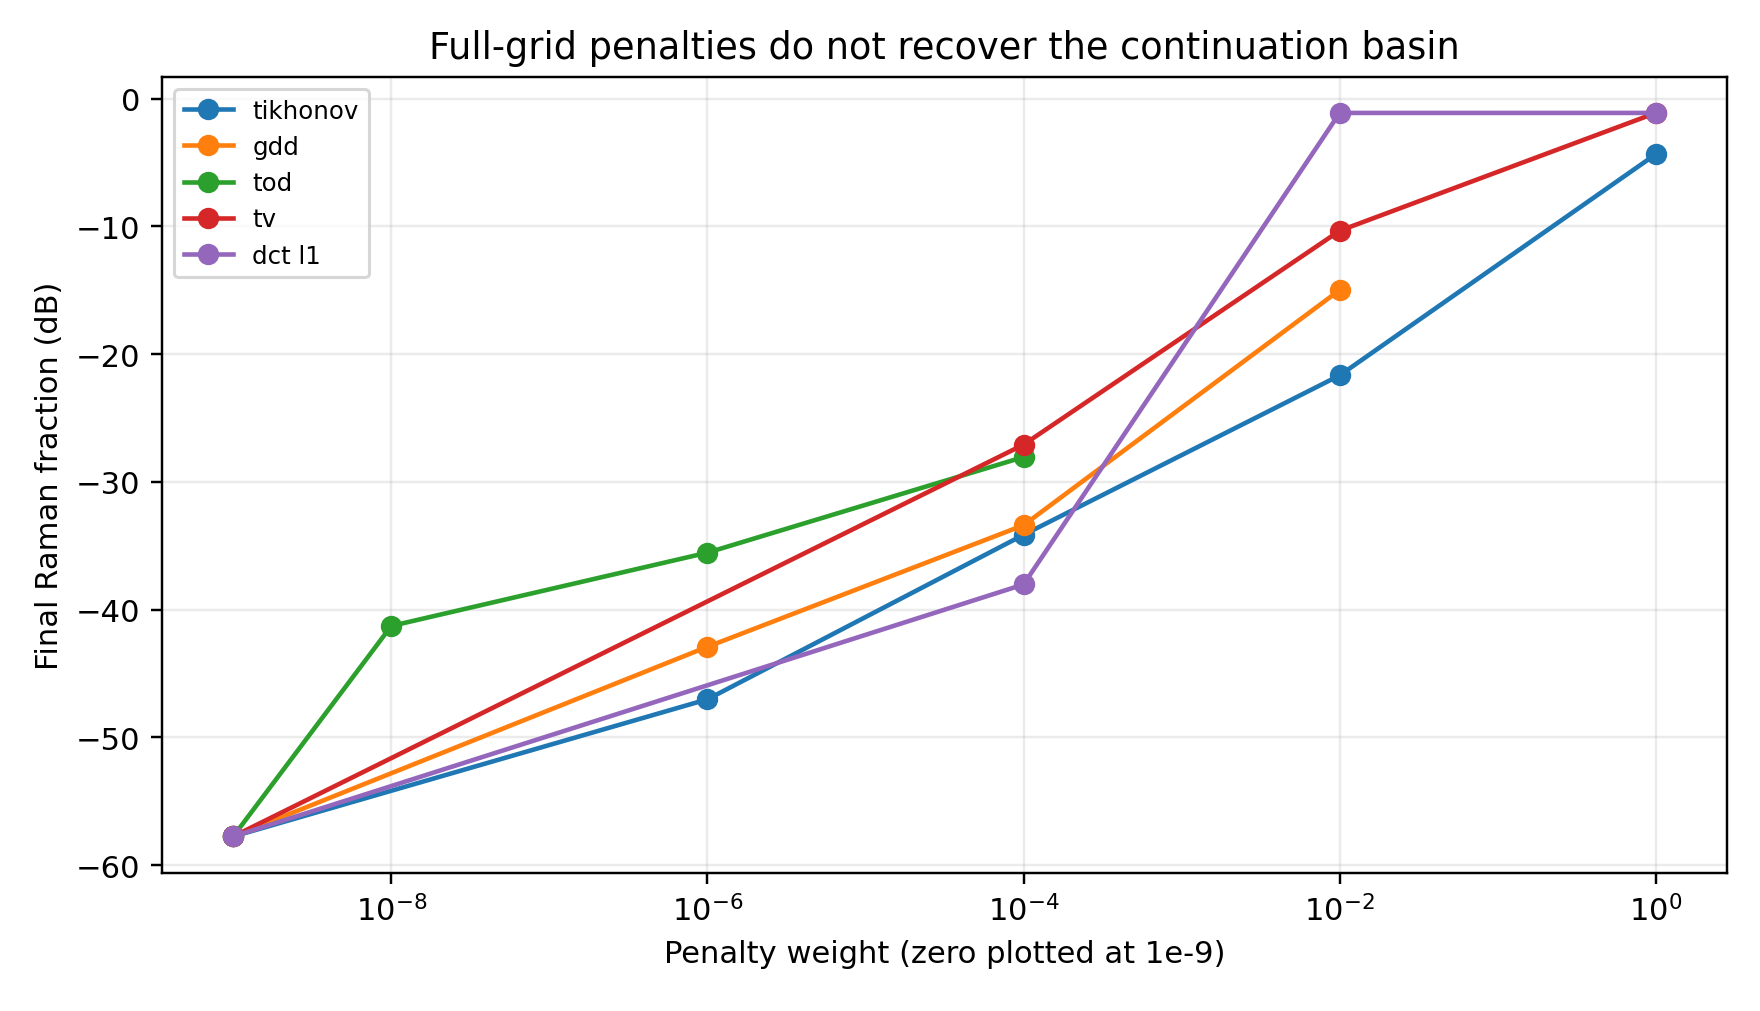
\includegraphics[width=0.9\linewidth]{figures/regularization_penalty_scan.png}
\caption{Full-grid regularization does not recover the best continuation basin.
Increasing penalty weight mostly trades away suppression; the unregularized
zero-start full-grid run remains about \(10\,\mathrm{dB}\) shallower than the
best continuation path.}
\end{figure}

\section{Result Provenance and Reproducibility}

The result numbers in this note come from saved local artifacts, not from
manual transcription. The full-grid refinement table is backed by the note
sidecar CSV in the local \texttt{tables/} directory.
The transfer and robustness numbers were cross-checked against the stability
summary sidecar used to build the standard diagnostics. The PDF copies only the
durable note-ready figures into this directory so the document can be read
without browsing internal result folders.

\begin{center}
\footnotesize
\begin{tabular}{@{}>{\raggedright\arraybackslash}p{0.16\linewidth}
                >{\raggedright\arraybackslash}p{0.33\linewidth}
                >{\raggedright\arraybackslash}p{0.30\linewidth}
                >{\raggedright\arraybackslash}p{0.12\linewidth}@{}}
\toprule
\textbf{Evidence} & \textbf{What it supports} & \textbf{Note-local files} & \textbf{Audit} \\
\midrule
Basis sweep &
Reduced-basis runs across polynomial, chirp-ladder, DCT, linear, and cubic
families. &
Depth summary; \texttt{cubic128\_reduced\_*}; \texttt{cubic32\_reduced\_*}. &
Checked locally. \\
\addlinespace
Penalty sweep &
Full-grid zero-start runs with smoothness or sparsity penalties. &
Penalty scan. &
Checked locally. \\
\addlinespace
Transfer &
Phase-noise width estimates and cross-fiber transfer checks. &
Robustness/transfer plot; \texttt{transferable\_polynomial\_*}. &
Checked locally. \\
\addlinespace
Full-grid refinement &
Reduced-basis seeds polished with unrestricted full-grid L-BFGS and compared to
zero-start full-grid optimization. &
Refinement plot; table CSV; \texttt{cubic32\_fullgrid\_*};
\texttt{zero\_fullgrid\_*}. &
CSV checked. \\
\bottomrule
\end{tabular}
\captionof{table}{Public provenance map for the reduced-basis note. The table
uses note-local filenames instead of internal run-folder names.}
\end{center}

The current reproducibility gap is packaging. The saved artifacts and
note-local figures exist, but there is not yet one clean public command that
regenerates the basis sweep, penalty sweep, transfer checks, and full-grid
refinement in one reproducible workflow. Until that workflow exists, this note
should cite the sidecar tables and copied standard images rather than
pretending that the whole result series is one clean public rerun workflow.

\subsection*{TL;DR}

The evidence is real, but the packaging is not finished. A reader can inspect
the copied figures and sidecar tables now; a future pass should add a clean
rerun command with public-facing names.

\subsection*{Reproduction Checklist}

A public rerun should produce, in order:
\begin{enumerate}
    \item the basis-family depth summary from the same SMF-28, \(2\,\mathrm{m}\),
    \(0.2\,\mathrm{W}\), \(\Nt=16384\) benchmark;
    \item the penalty-sweep comparison showing that zero-start full-grid
    regularization does not reach the continuation basin;
    \item the transfer and robustness table with \(\JdB\), \(\sigmathreedb\),
    and HNLF gap for each selected candidate;
    \item the full-grid refinement table showing continuation-seeded runs
    compared with the zero-start full-grid baseline;
    \item a standard image set for every selected phase: phase diagnostic,
    shaped evolution heat map, phase profile, and unshaped evolution reference.
\end{enumerate}

If any rerun changes a table value by more than normal numerical tolerance, the
figures and sidecar tables in this note should be regenerated together.

\clearpage
\section{Paired Diagnostics and Heat Maps}

Each visual case below puts the phase diagnostic and the matching propagation
heat map on the same page. The diagnostic shows what phase shape the optimizer
found. The heat map shows how the spectrum evolves along the fiber. The two
images need to be read together.

\subsection*{How To Read These Pages}

\textbf{Phase diagnostic.} This is the input control: wrapped phase, unwrapped
phase, group delay, group-delay dispersion, and instantaneous frequency shift.
Smooth structure usually means the mask is easier to explain and implement;
rapid oscillations usually mean more fragile control.

\textbf{Spectral-evolution heat map.} This is the fiber response. It shows how
spectral power moves along propagation length after the phase mask is applied.

\textbf{Control comparison.} The no-optimization page is the control group.
The deep cubic pages show basin access. The polynomial page shows
transferability. The full-grid refinement page shows whether the reduced seed
survives after the basis restriction is removed.

\subsection*{Intuition Check}

The phase diagnostic answers ``what did we tell the input pulse to do?'' The
heat map answers ``what did the fiber actually do with that input?'' A reduced
basis result needs both images because the basis shape and the propagation
response are different pieces of evidence.

\clearpage

\subsection*{Control Reference: No Optimization}

\begin{figure}[H]
\centering
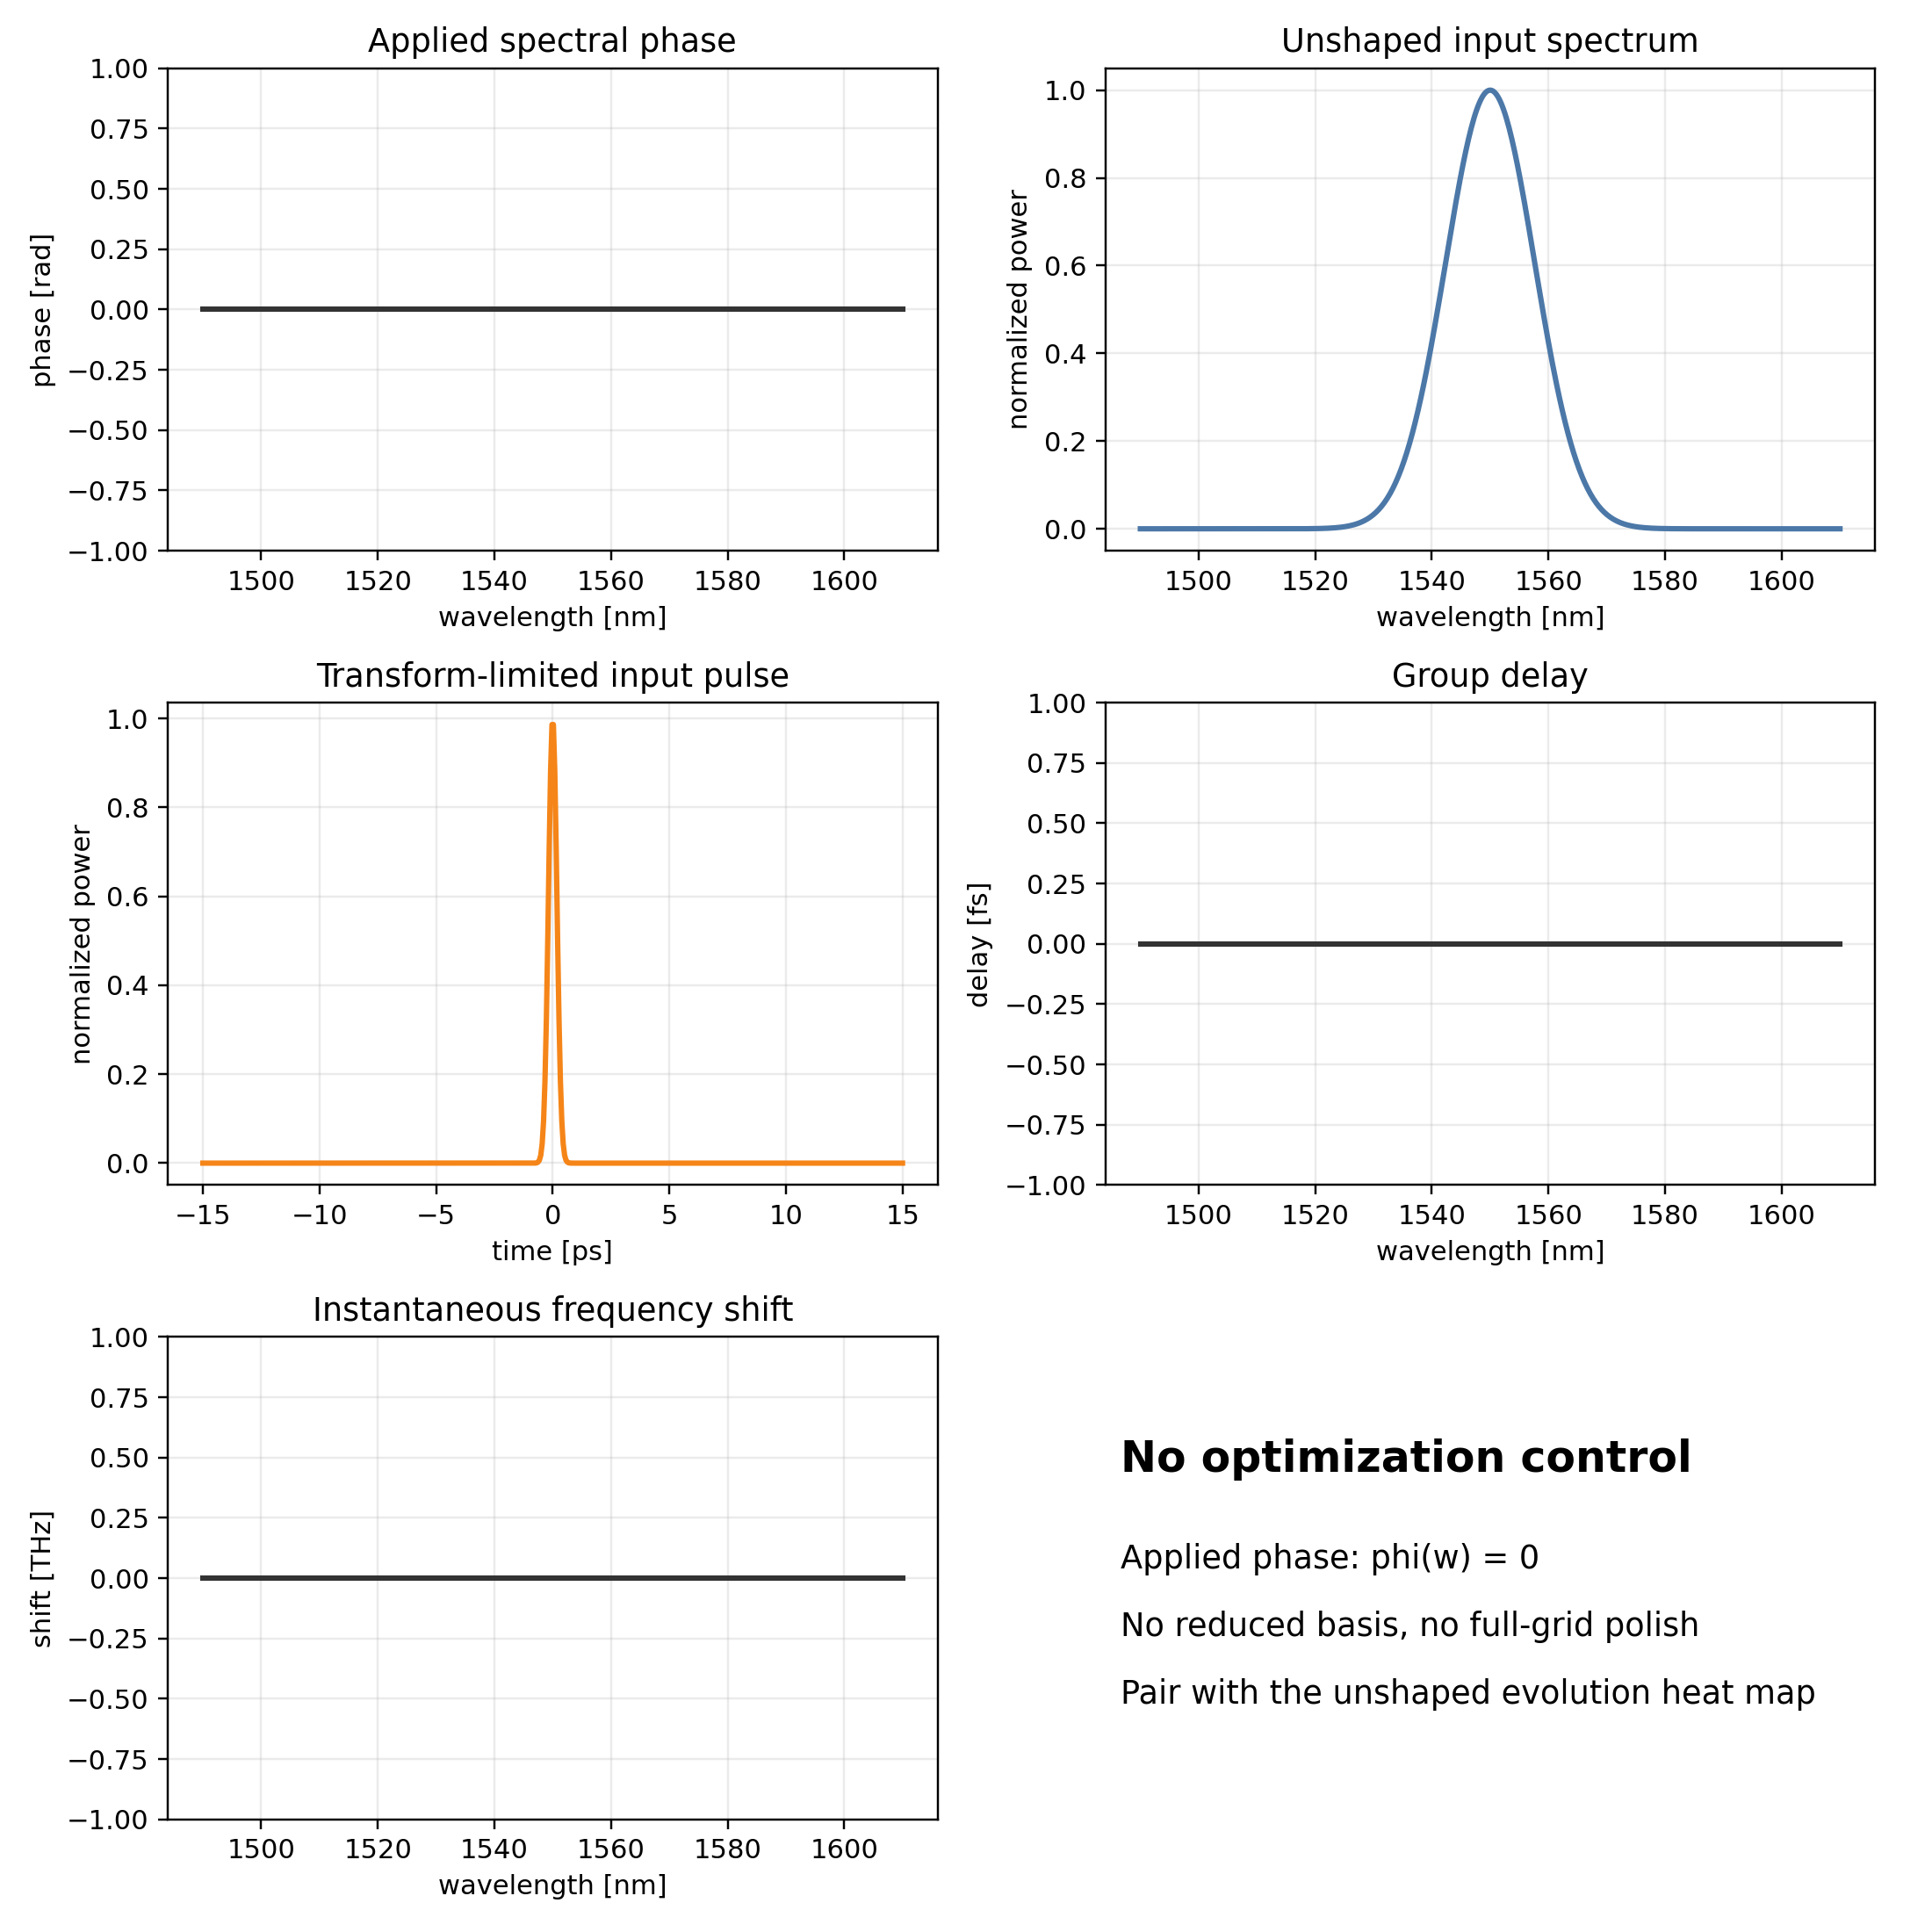
\includegraphics[height=0.47\textheight]{figures/no_optimization_phase_diagnostic.png}
\vspace{0.5em}

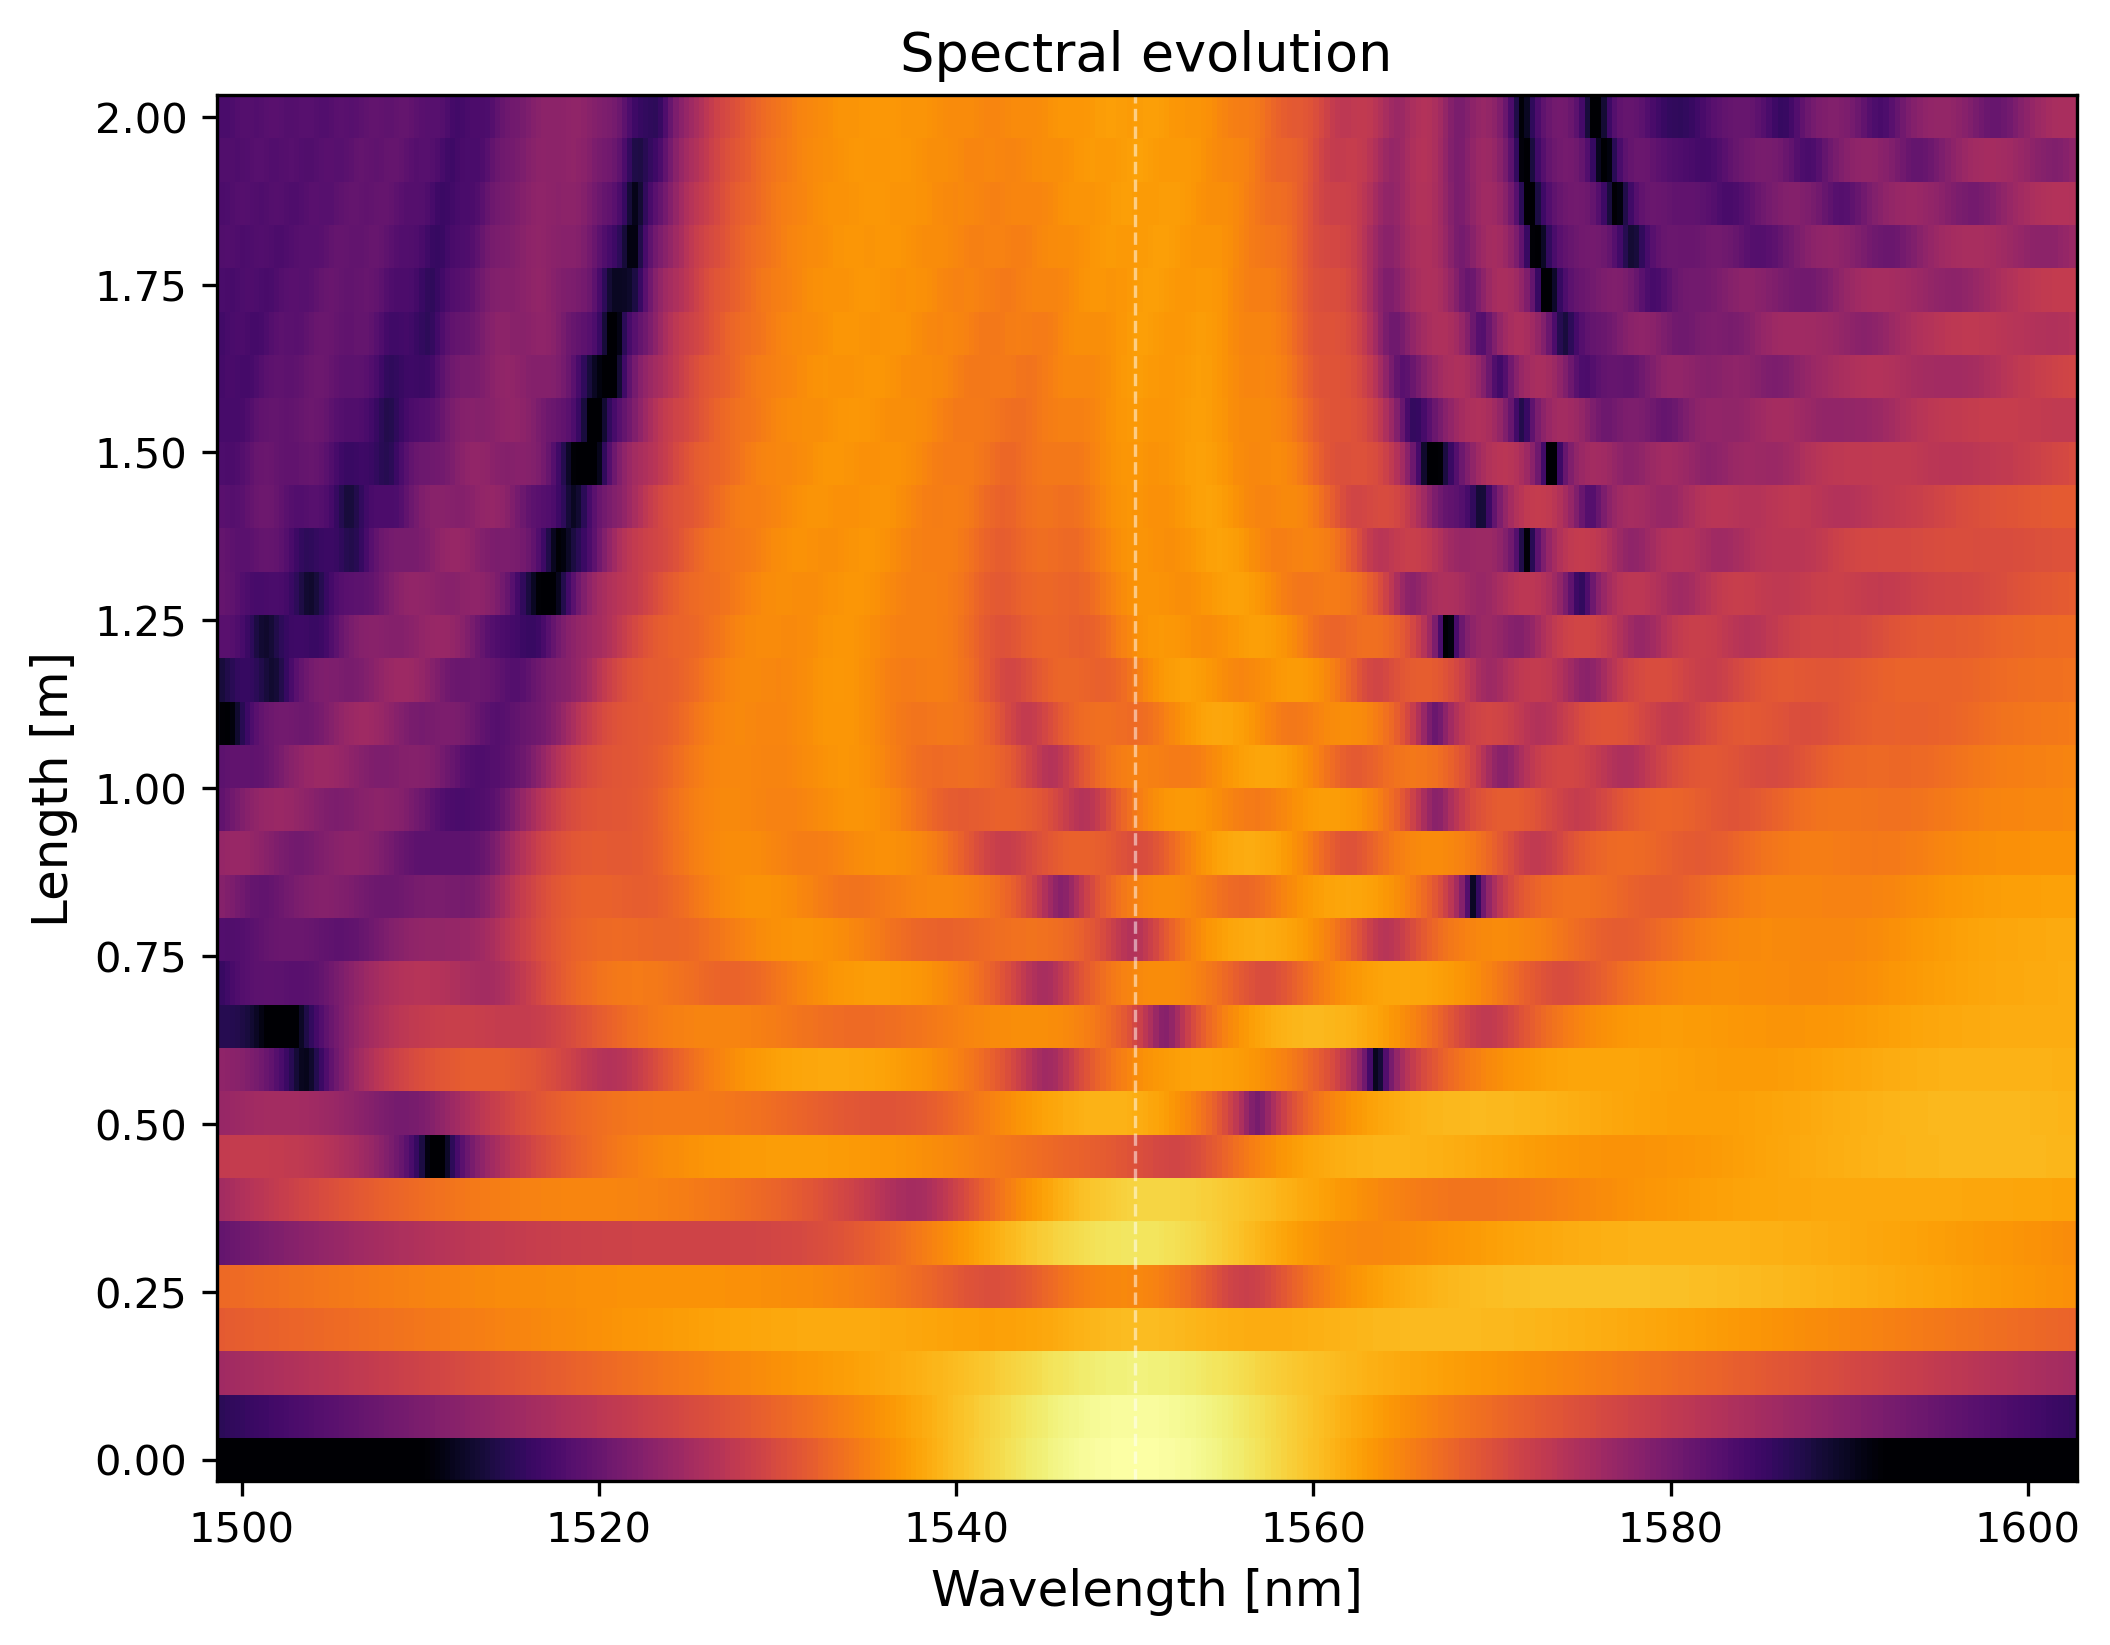
\includegraphics[height=0.31\textheight]{figures/no_optimization_evolution_unshaped.png}
\caption{Control reference: no optimization and no applied spectral phase. This
page is the unshaped baseline. It shows what the system does before any reduced
basis, continuation, or full-grid polishing is allowed.}
\end{figure}

\clearpage
\subsection*{Deep Cubic Continuation}

\begin{figure}[H]
\centering
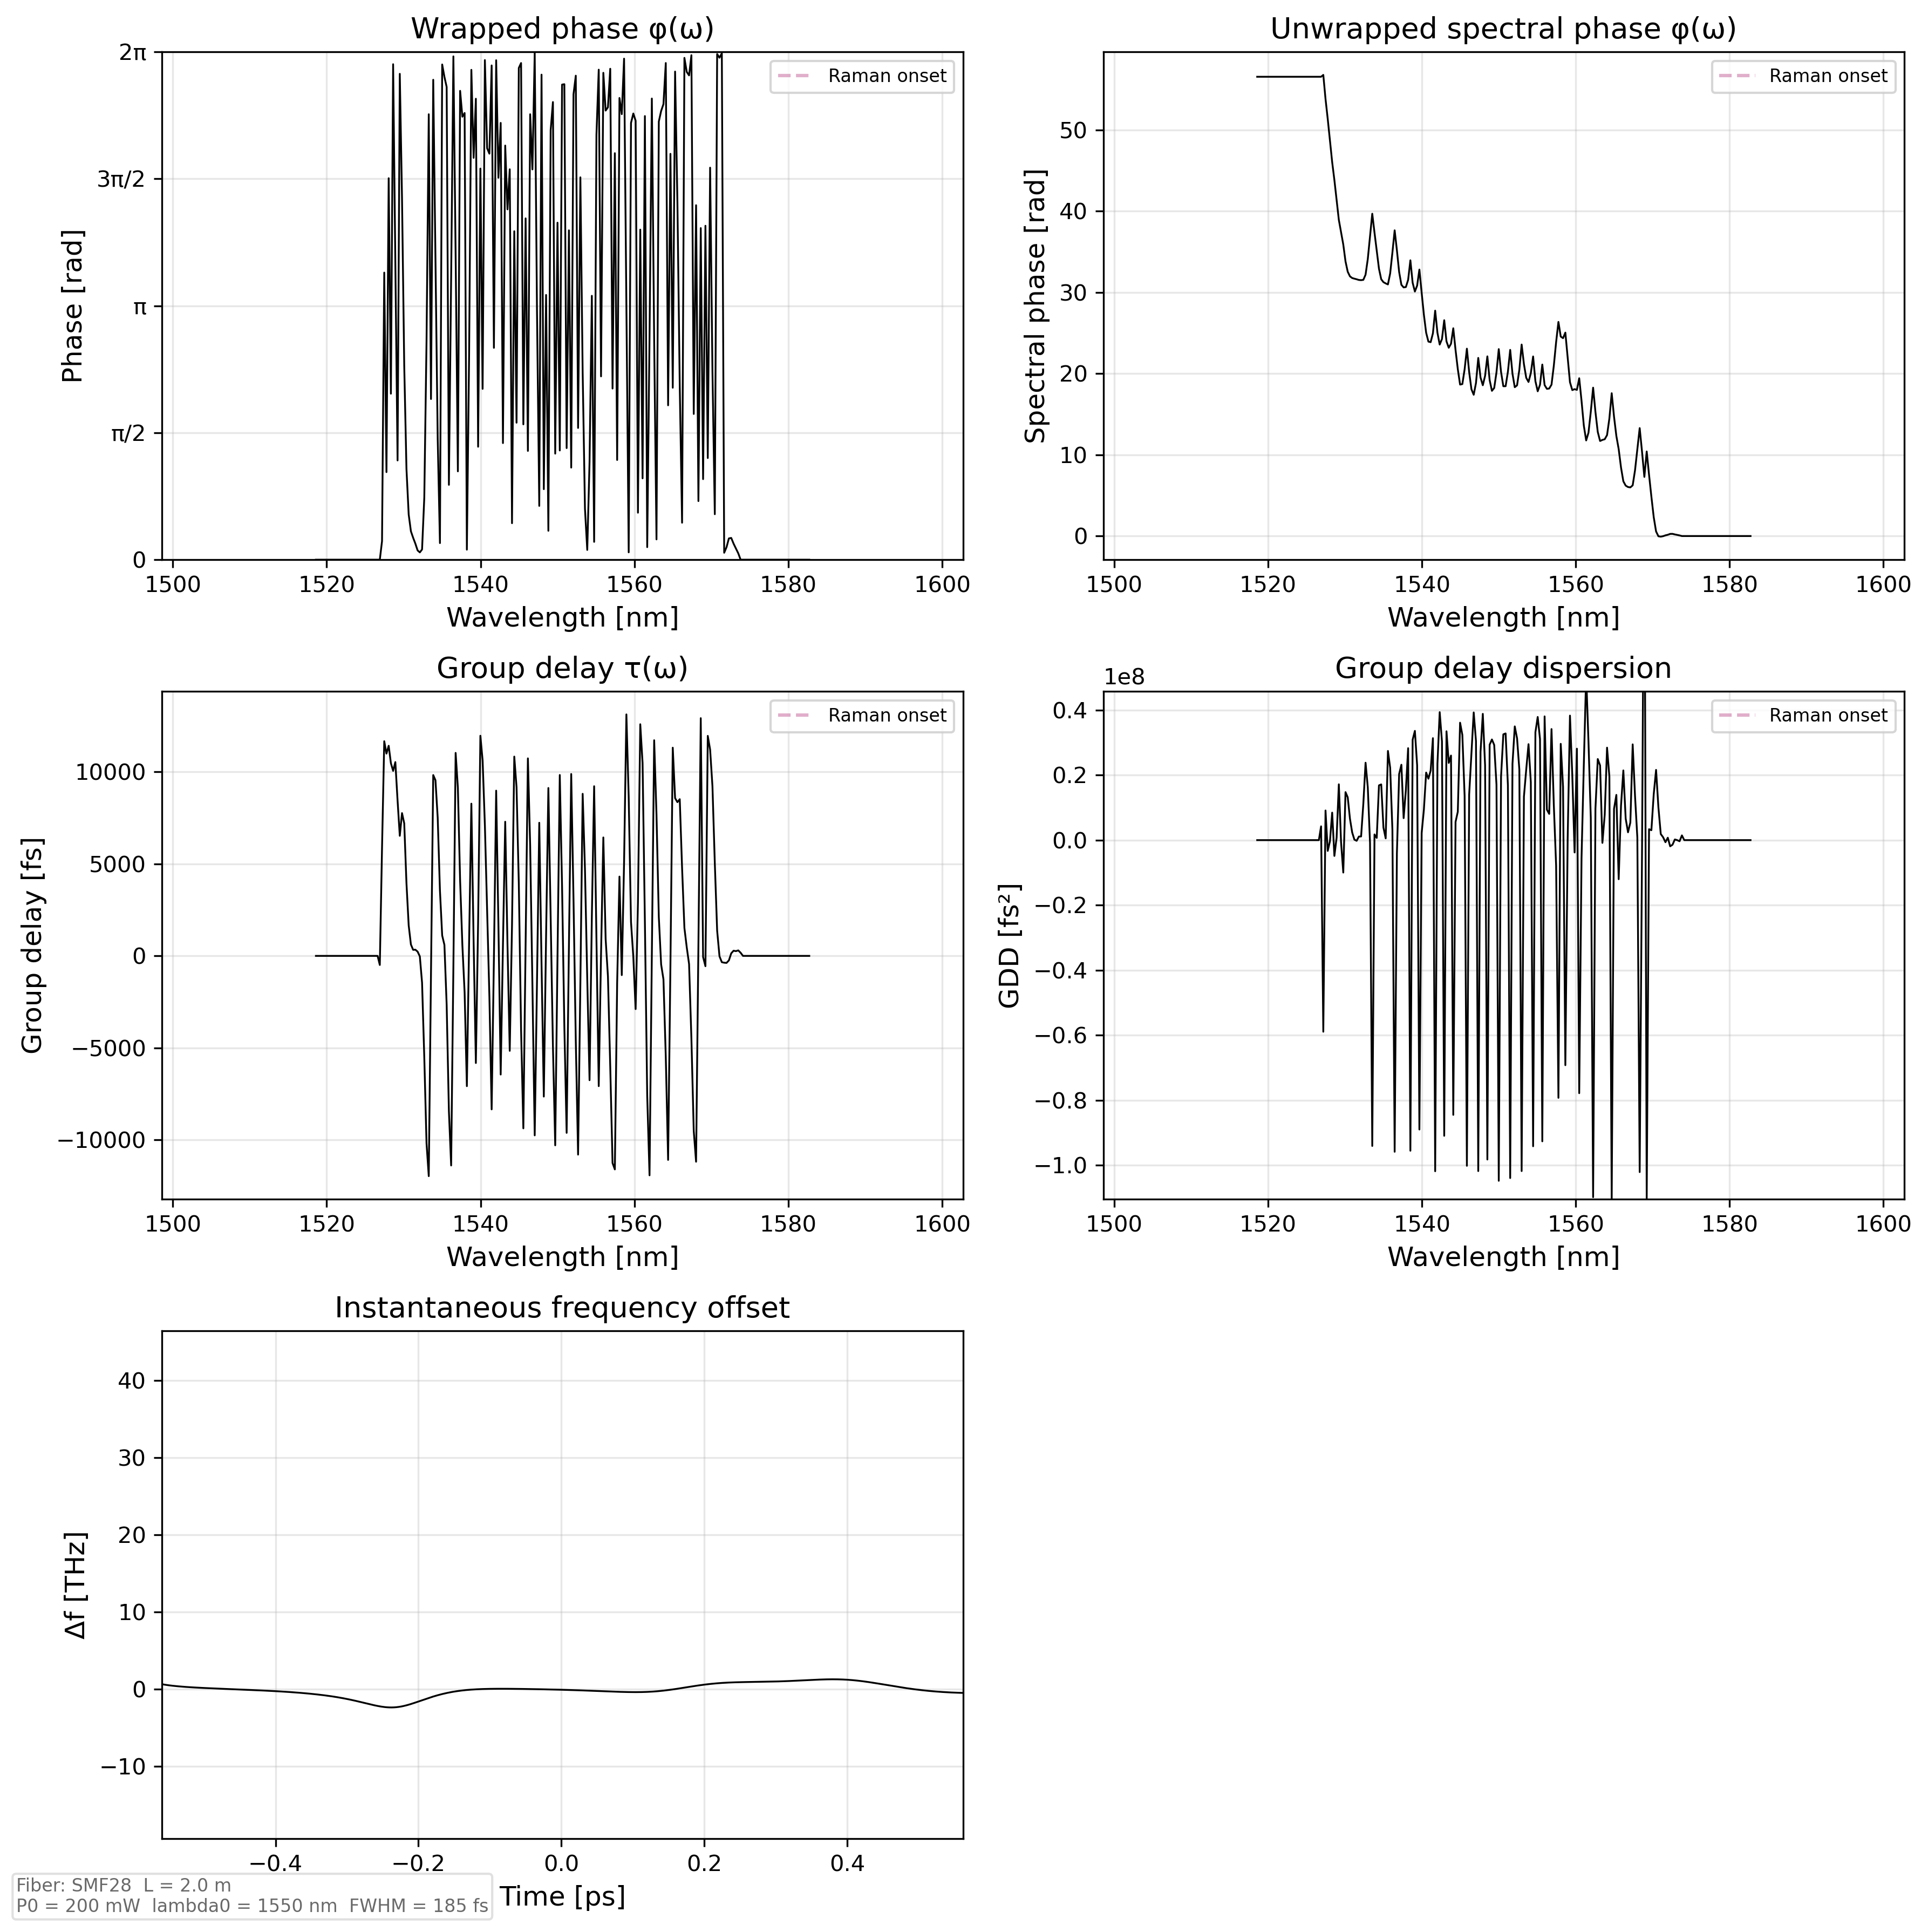
\includegraphics[height=0.47\textheight]{figures/cubic128_reduced_phase_diagnostic.png}
\vspace{0.5em}

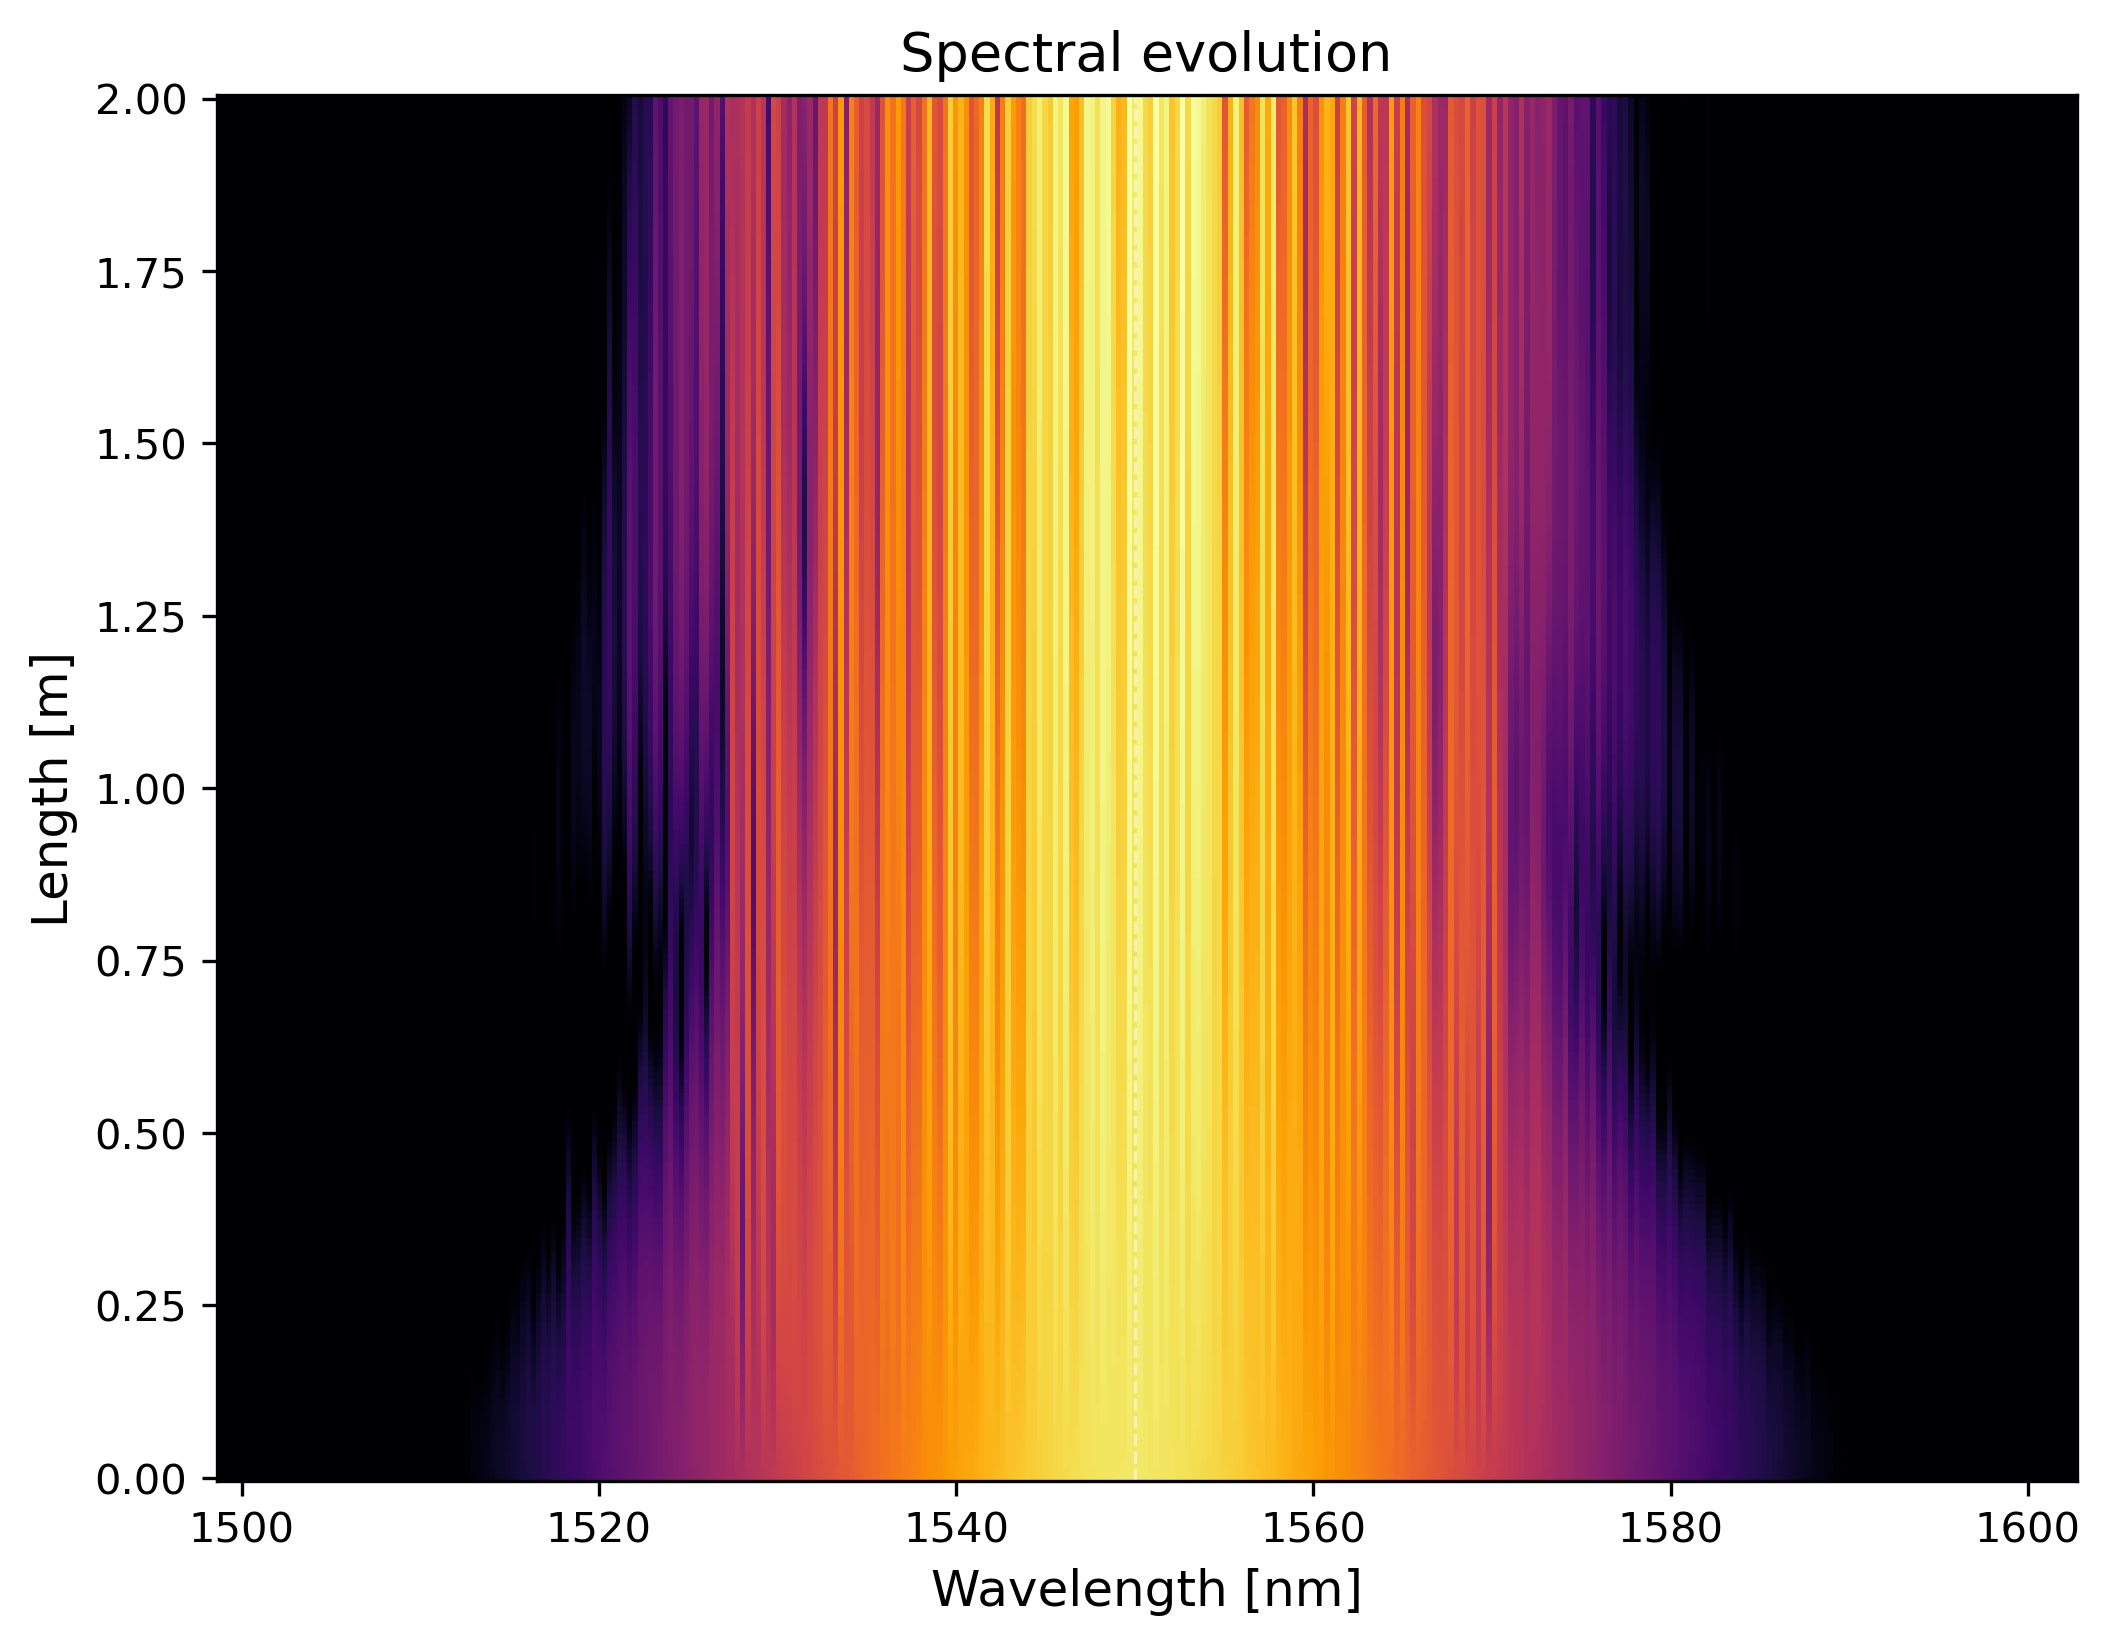
\includegraphics[height=0.31\textheight]{figures/cubic128_reduced_evolution.png}
\caption{Deep cubic-continuation case. This is the best canonical suppression
result in the reduced-basis sweep, but it is also narrow and fiber-specific.}
\end{figure}

\clearpage
\subsection*{Moderate Cubic Seed}

\begin{figure}[H]
\centering
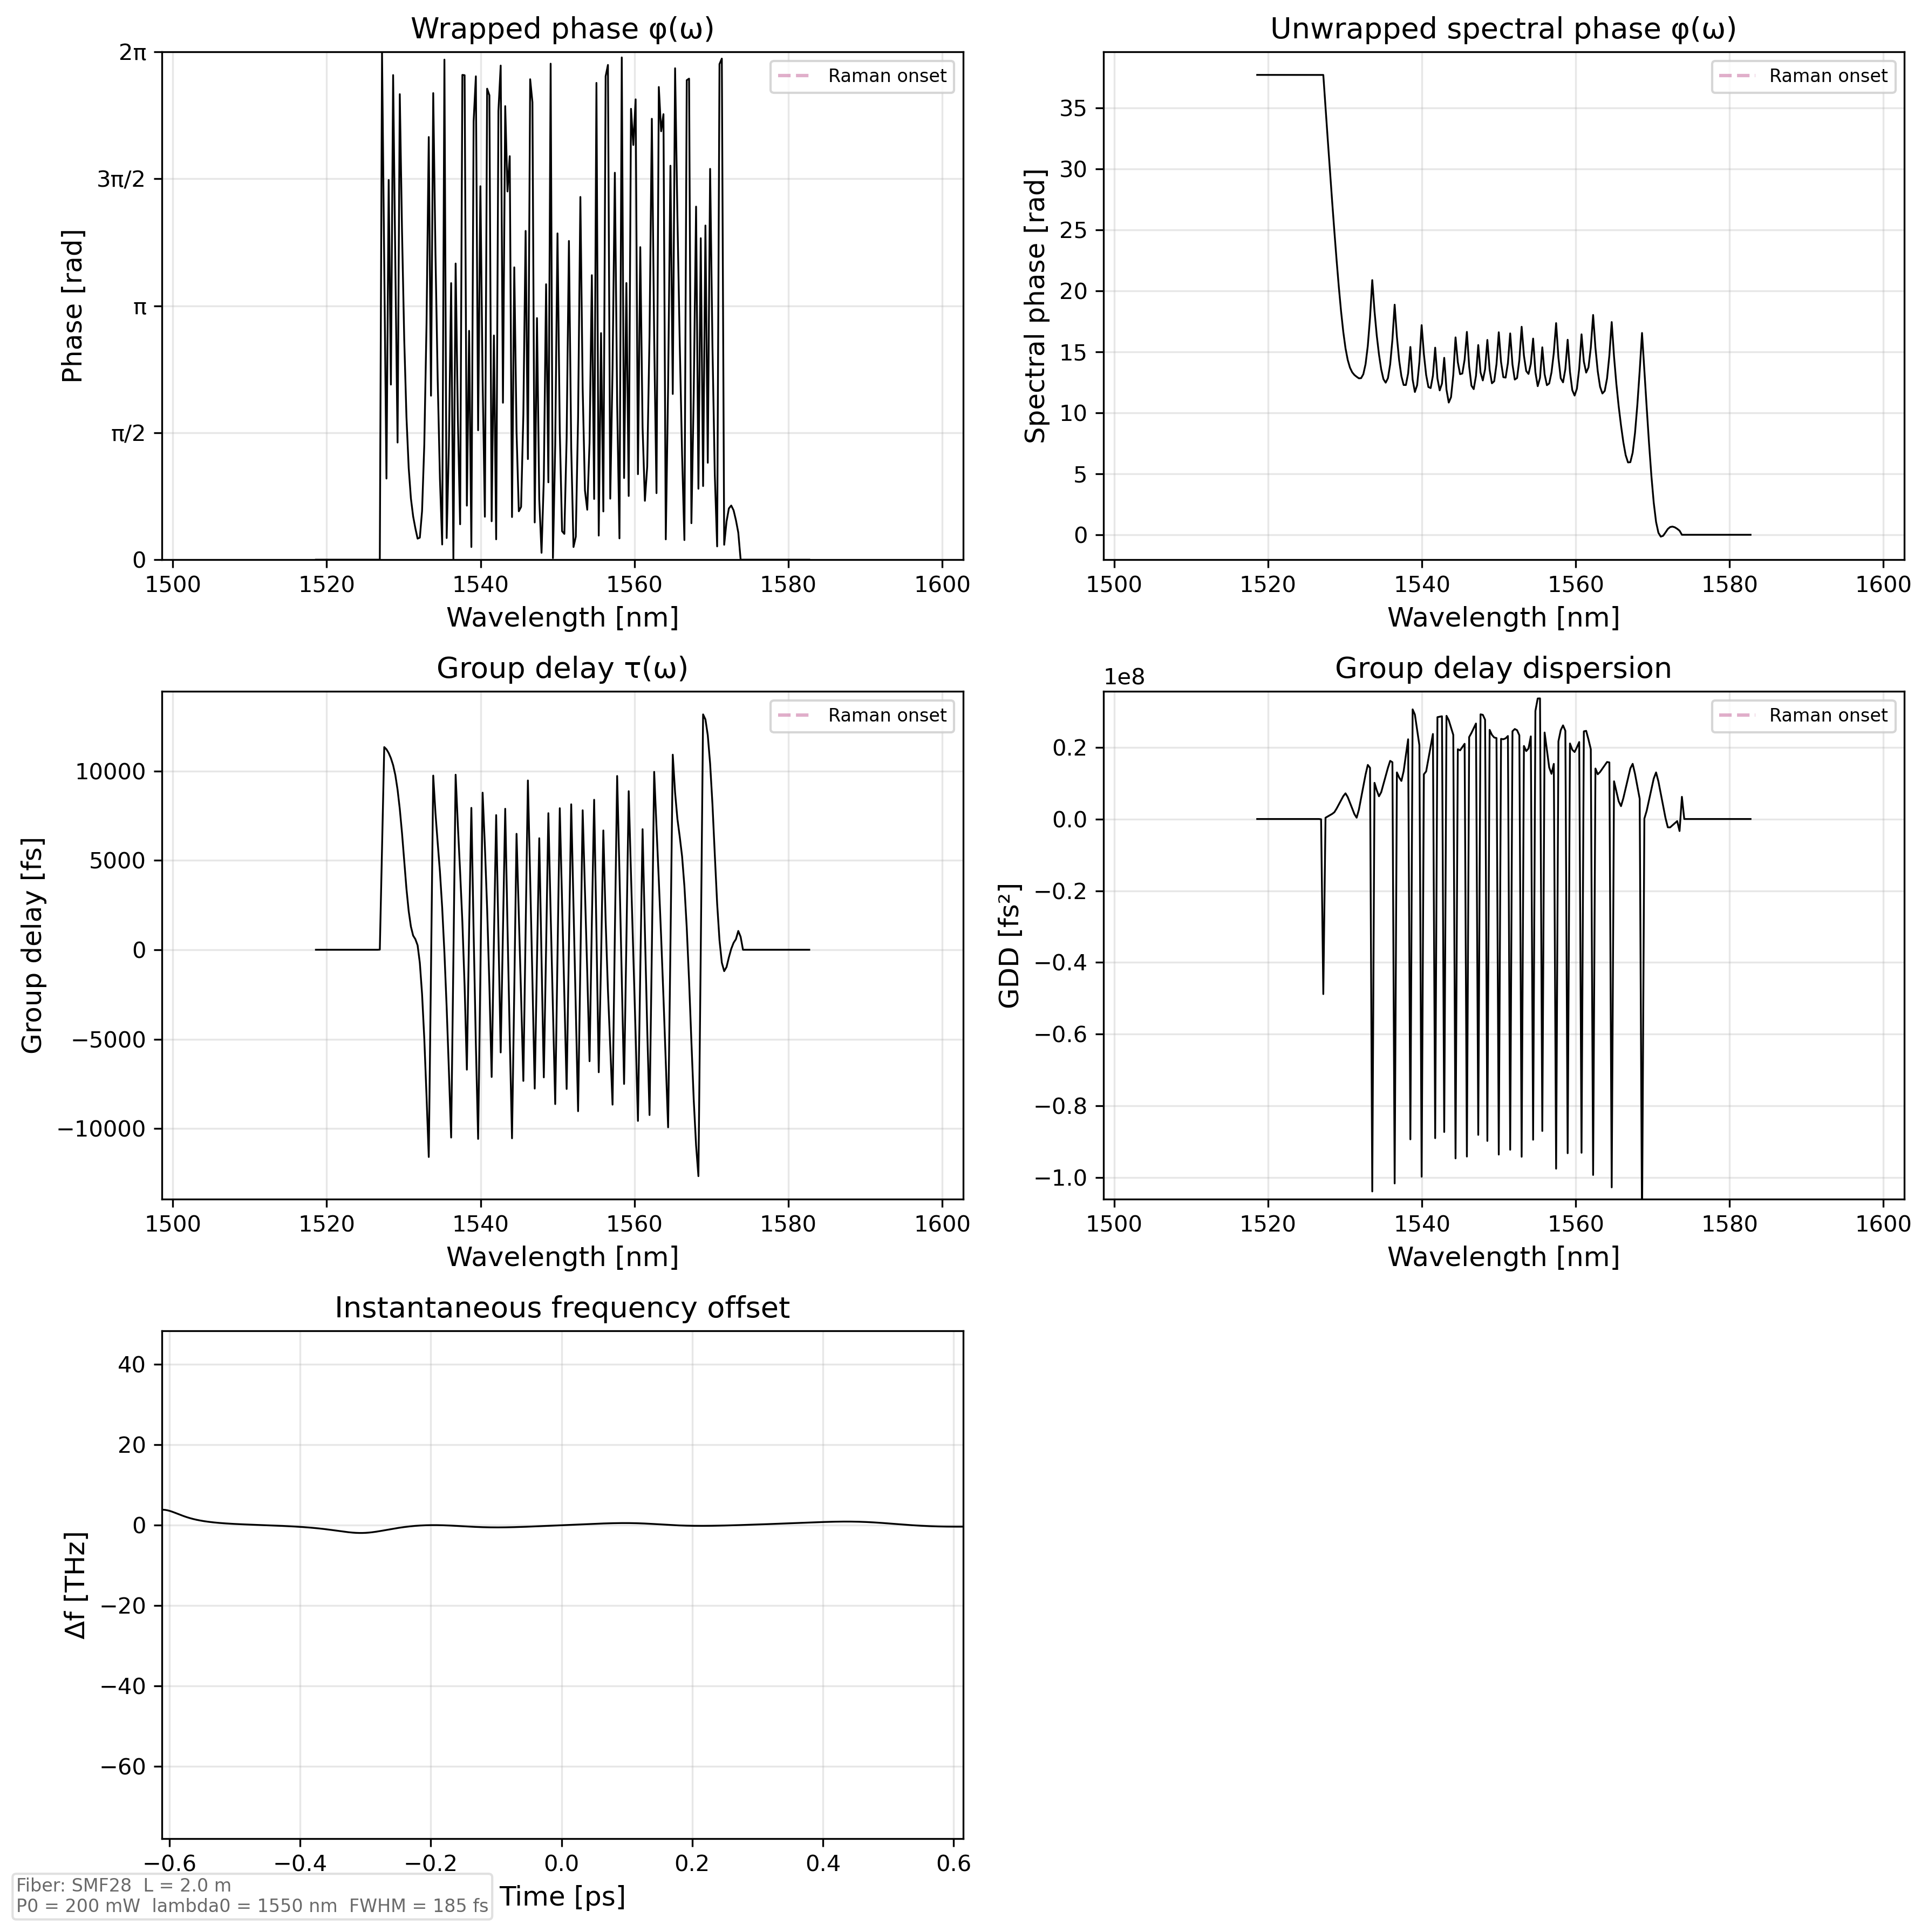
\includegraphics[height=0.47\textheight]{figures/cubic32_reduced_phase_diagnostic.png}
\vspace{0.5em}

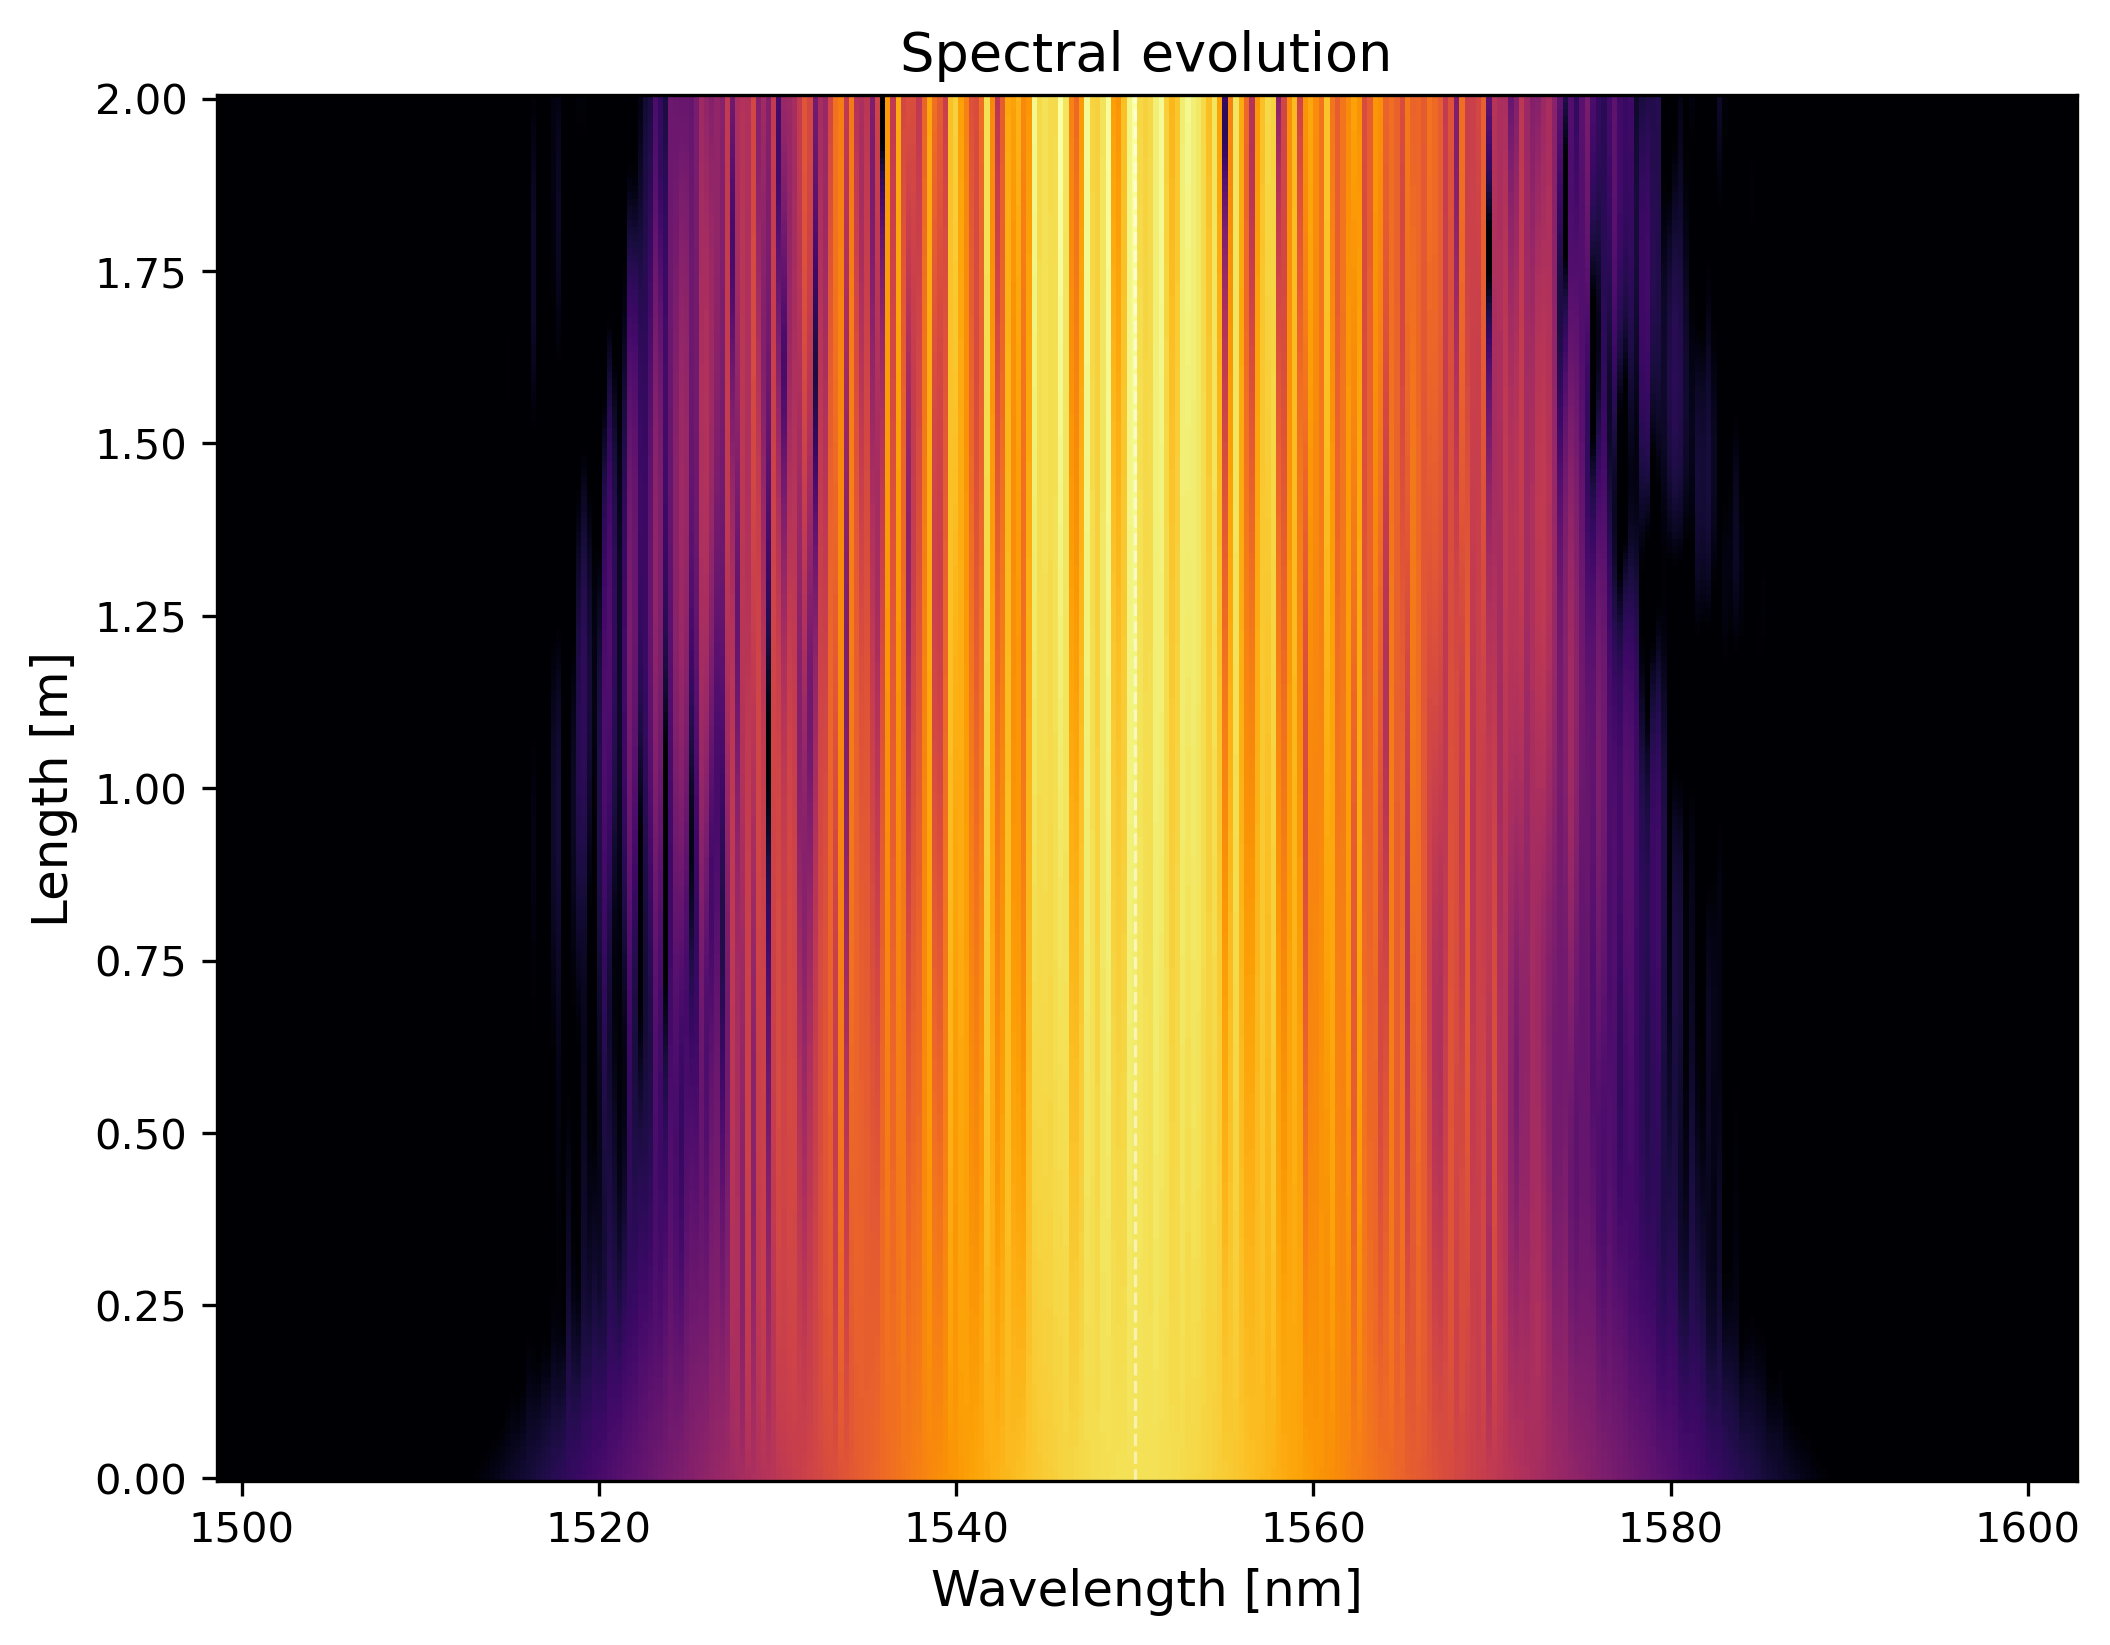
\includegraphics[height=0.31\textheight]{figures/cubic32_reduced_evolution.png}
\caption{Moderate cubic-continuation case. This result is not as deep before
full-grid refinement, but it is important because it can seed the deeper
full-grid family.}
\end{figure}

\clearpage
\subsection*{Transferable Polynomial Profile}

\begin{figure}[H]
\centering
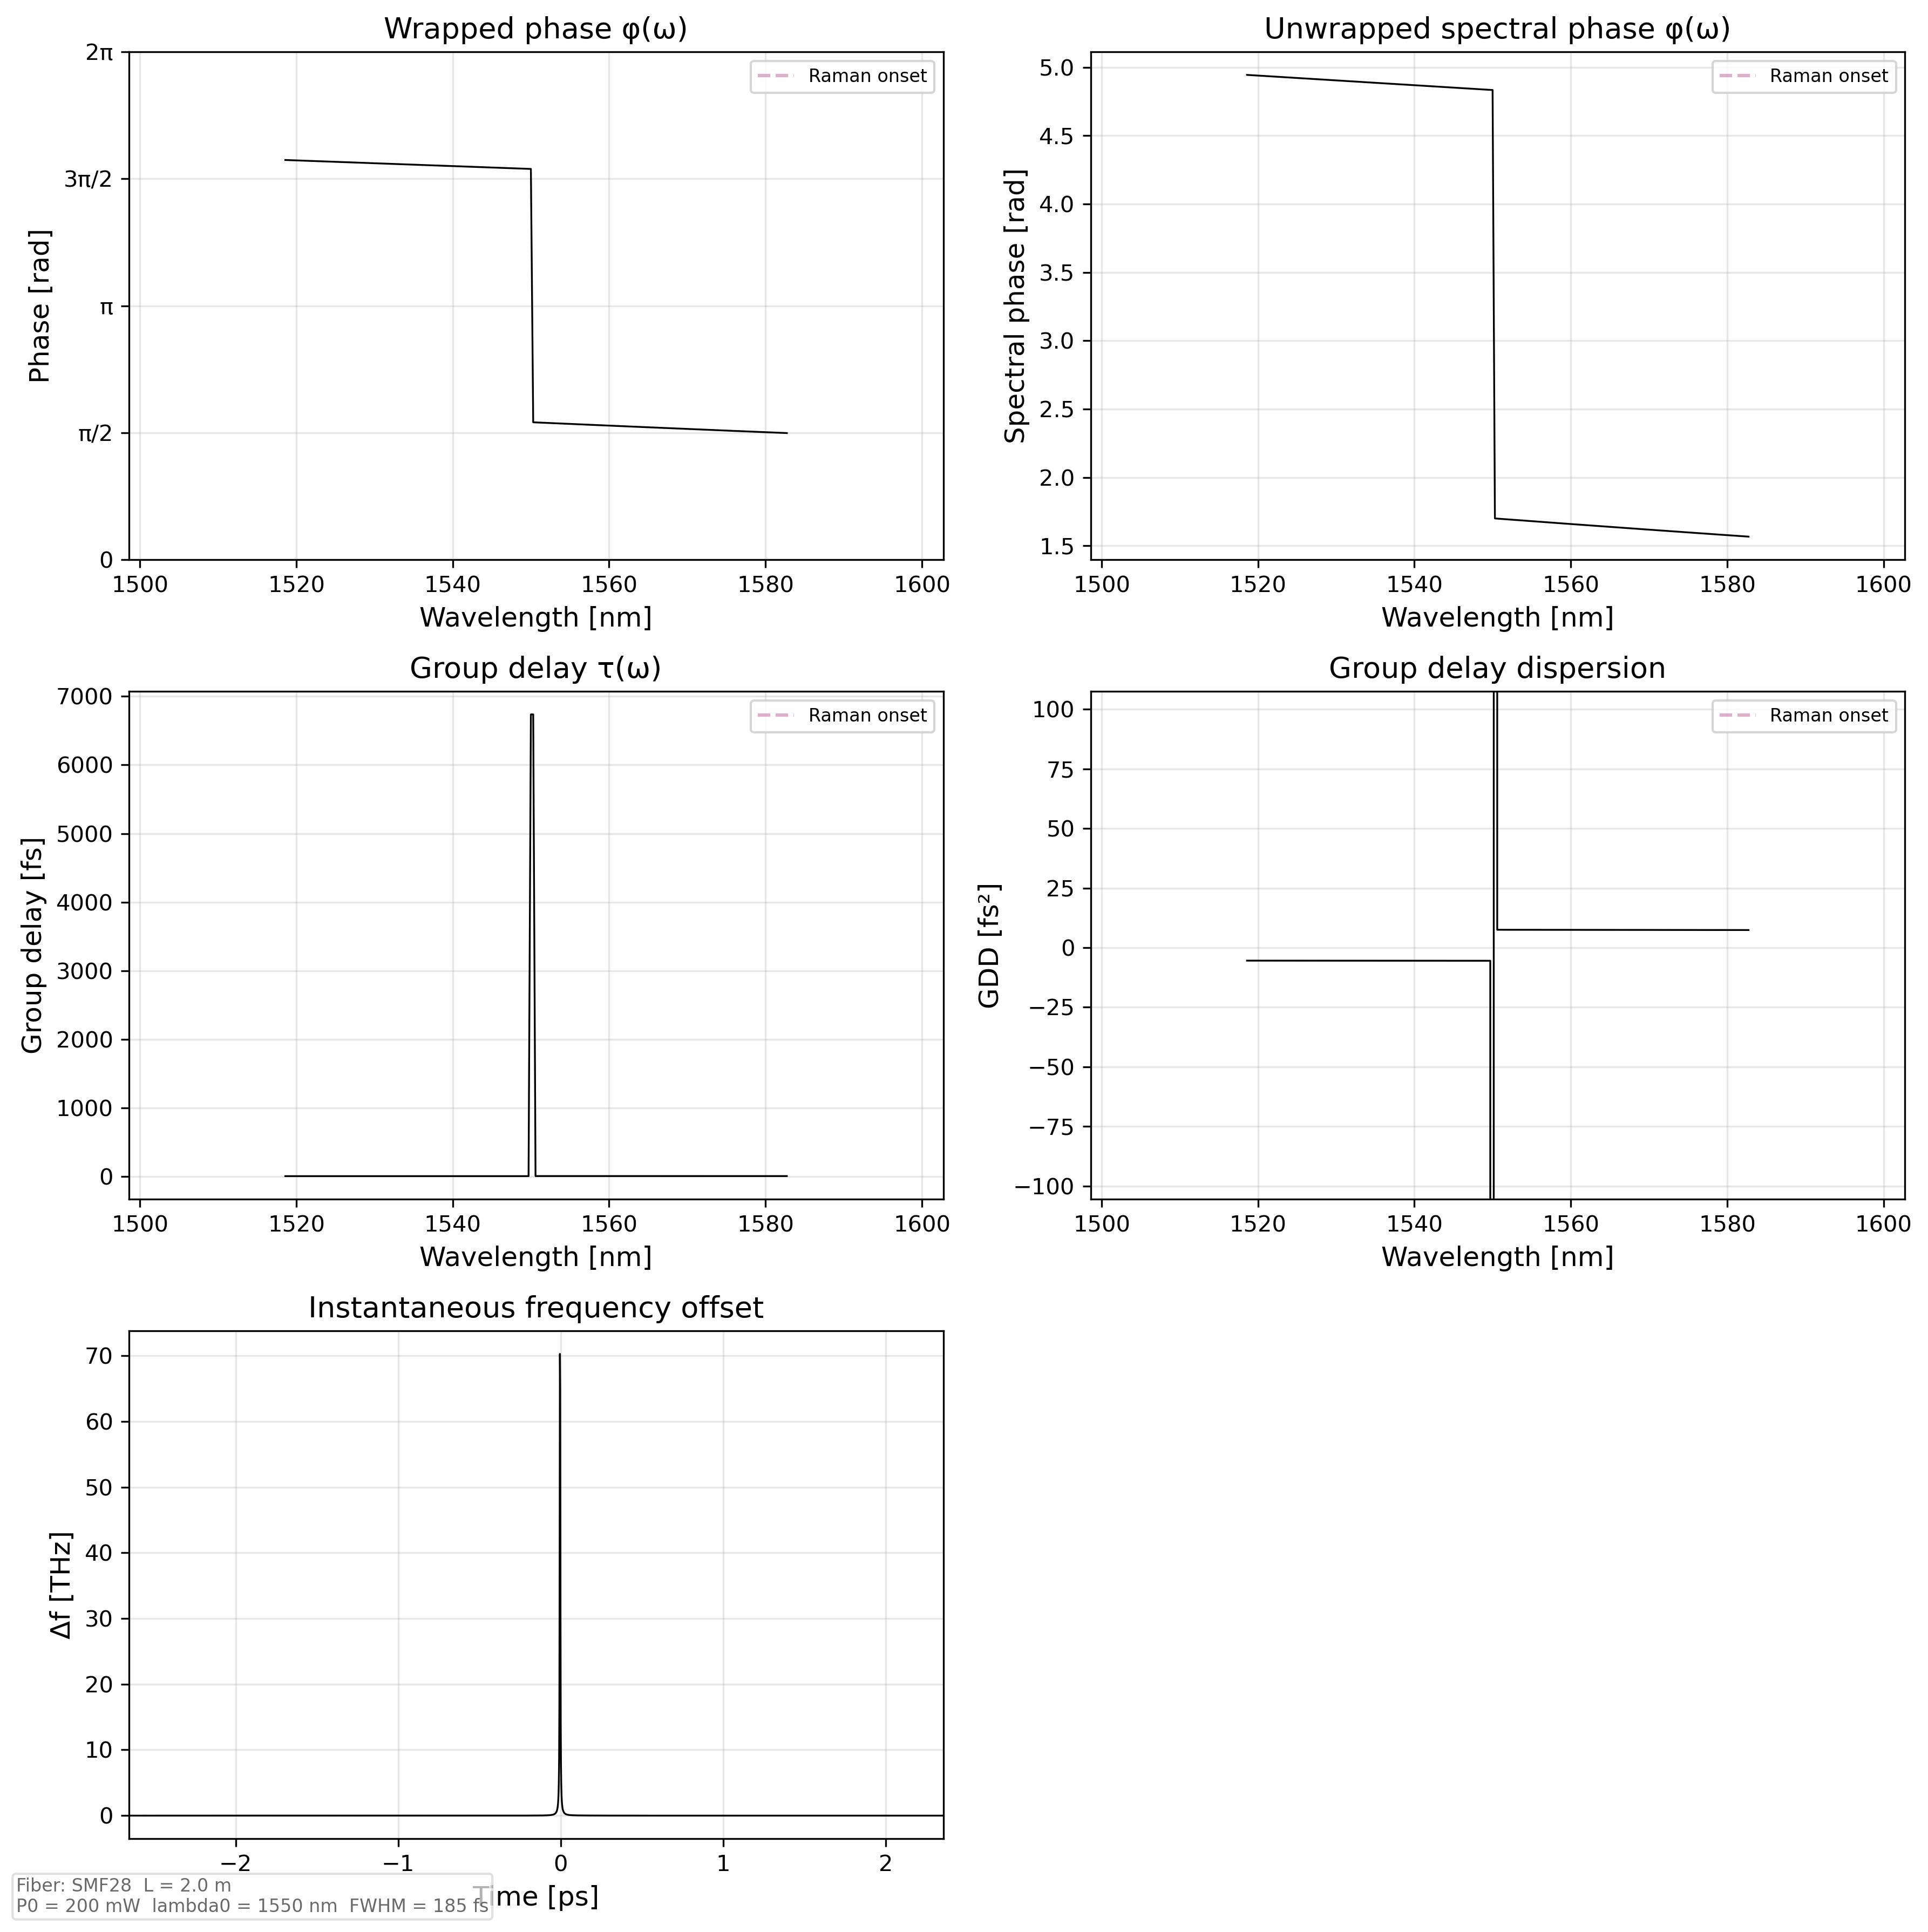
\includegraphics[height=0.47\textheight]{figures/transferable_polynomial_phase_diagnostic.png}
\vspace{0.5em}

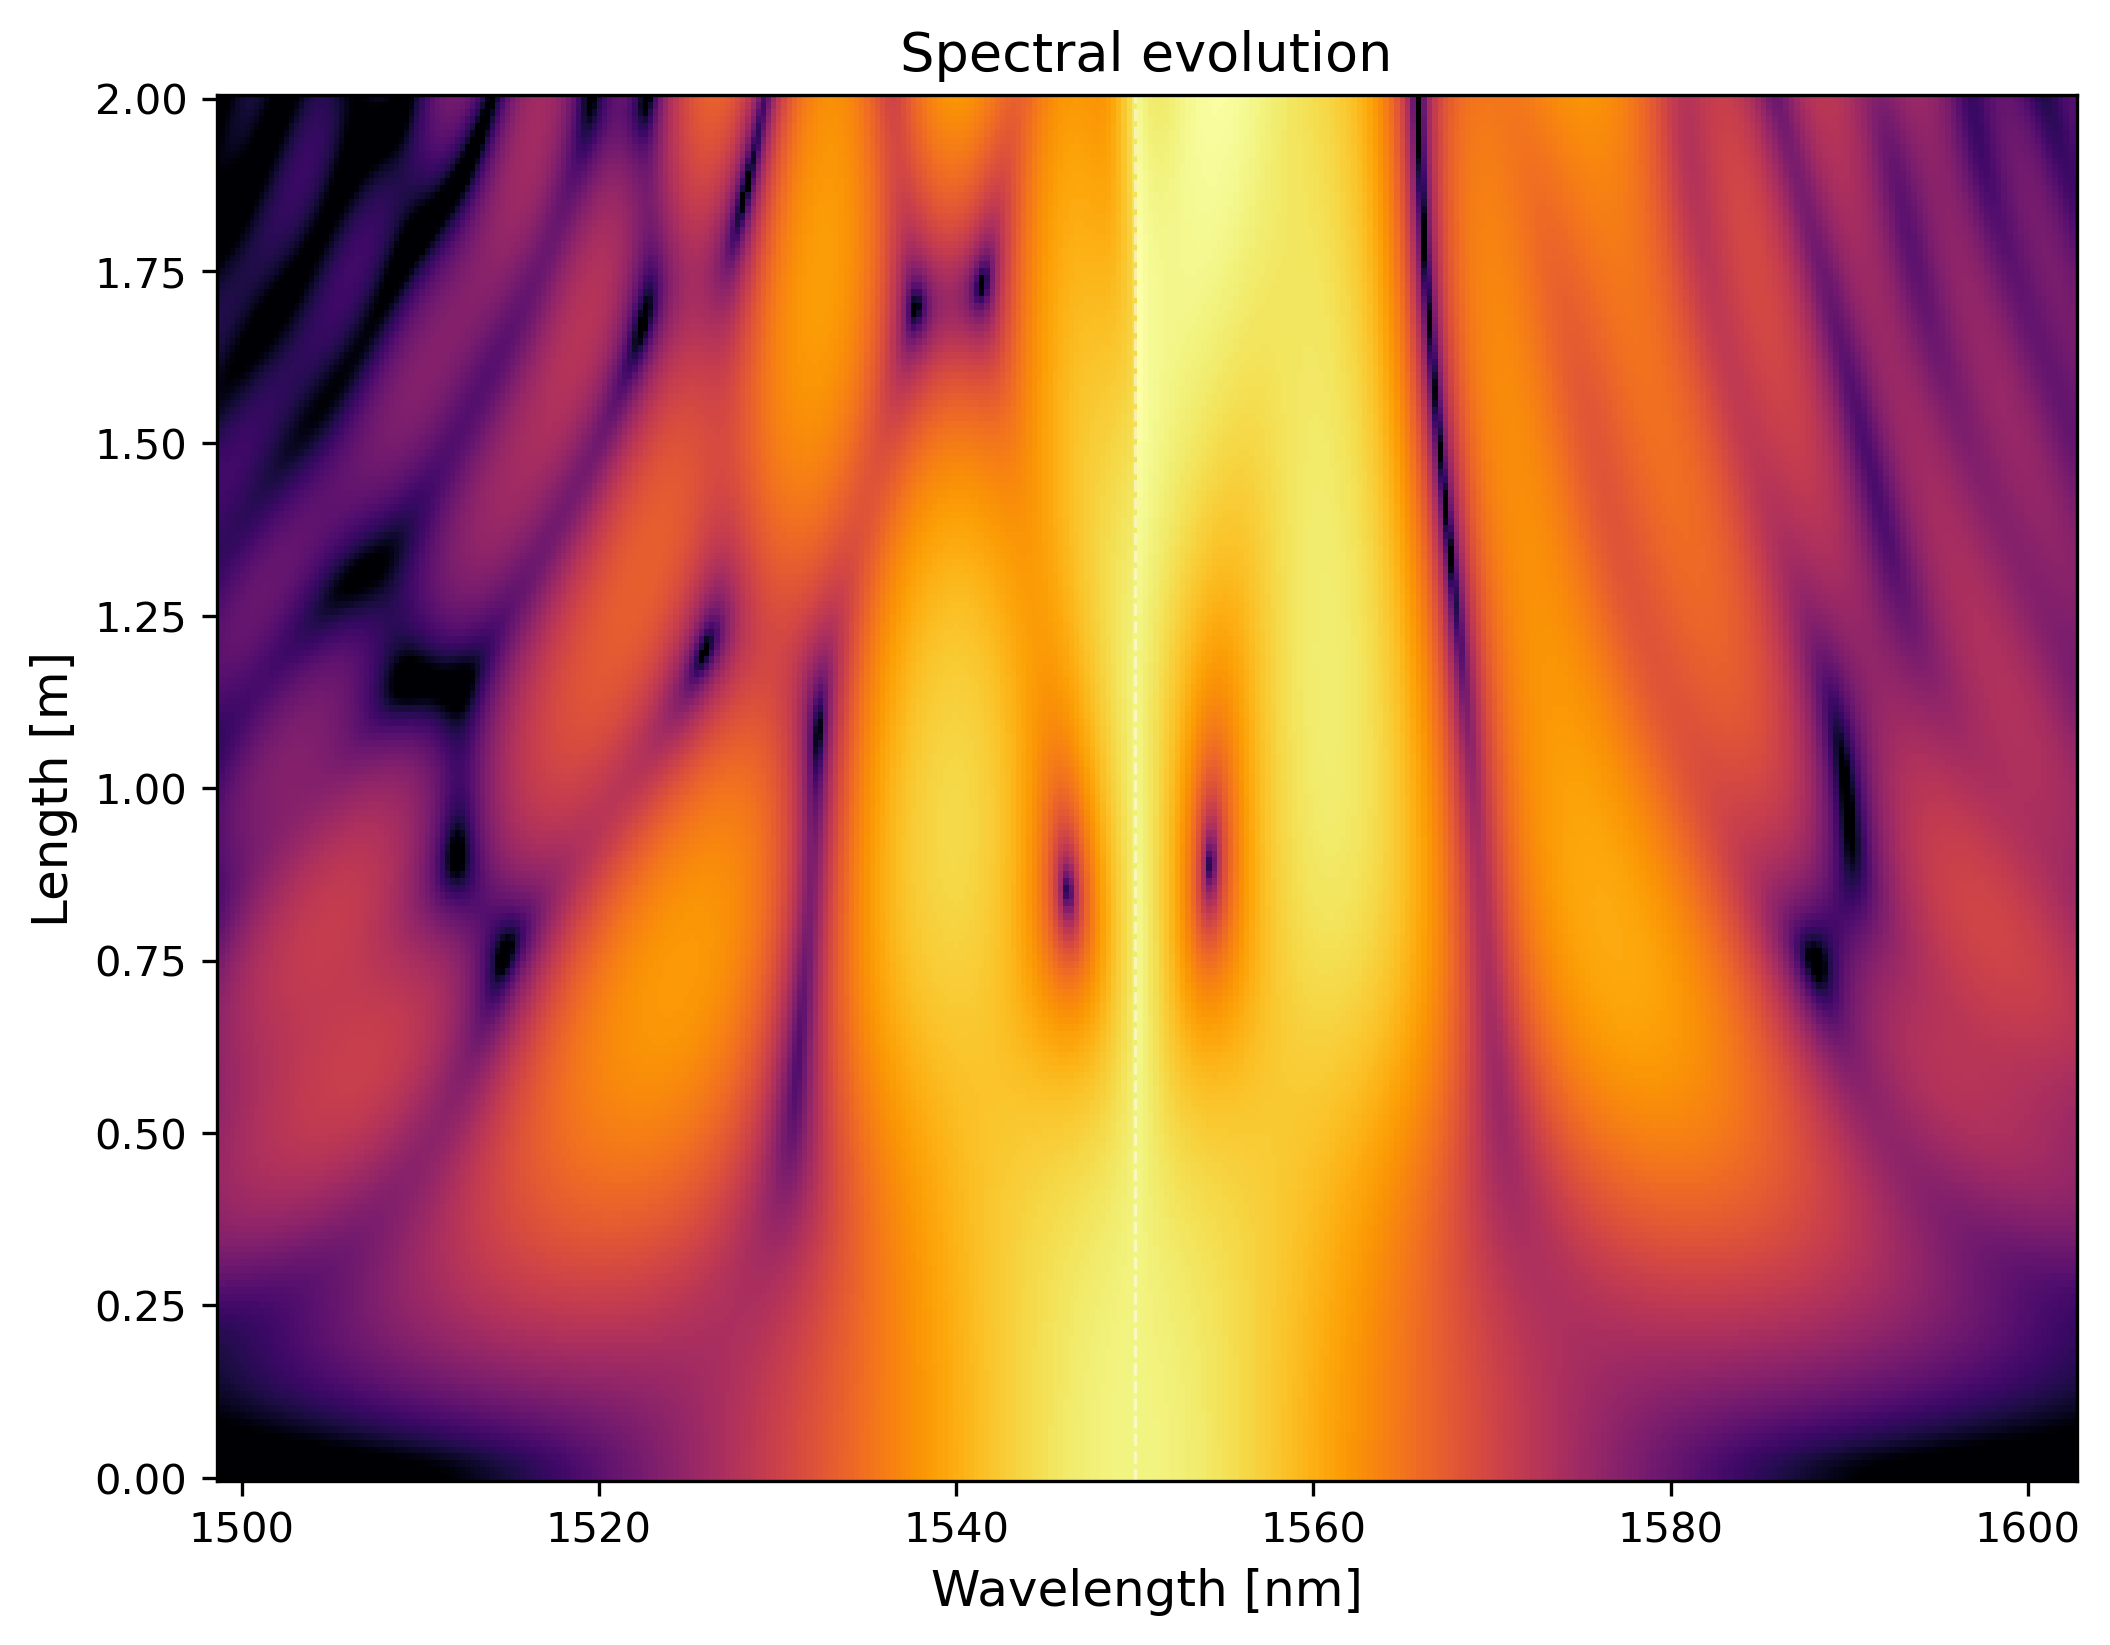
\includegraphics[height=0.31\textheight]{figures/transferable_polynomial_evolution.png}
\caption{Simple polynomial case. This is not the deepest solution, but it is
the cleanest transferable profile in this evidence set.}
\end{figure}

\clearpage
\section{Full-Grid Refinement Check}

The strongest possible objection is that a reduced-basis optimum might look good
only because the coordinate restriction hides descent directions. The follow-up
test seeded full-grid L-BFGS from selected reduced-basis optima.

\begin{figure}[H]
\centering
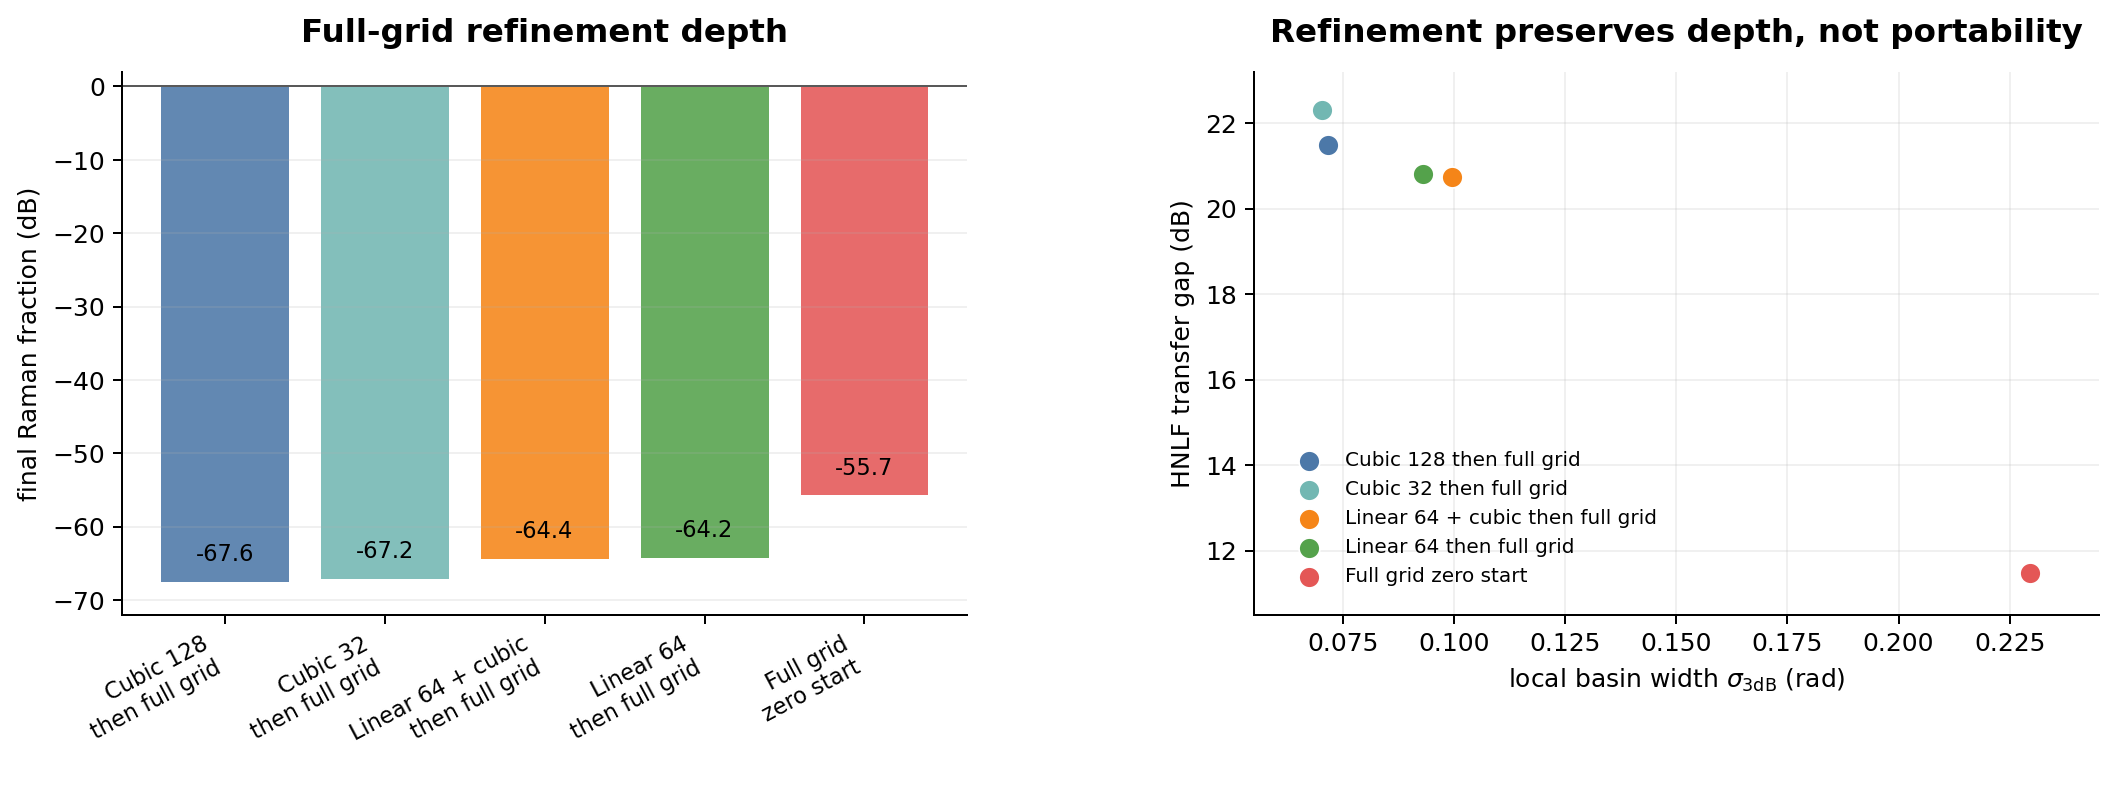
\includegraphics[width=0.92\linewidth]{figures/full_grid_refinement_paths.png}
\caption{Full-grid refinement preserves the depth of continuation-seeded
solutions, but does not fix their portability. The zero-start full-grid path has
the widest local basin and smaller HNLF gap, but is much shallower.}
\end{figure}

\begin{center}
\small
\begin{tabular}{l r r r r}
\toprule
Seed path & Final \(\JdB\) & \(\Delta\) vs seed & \(\sigmathreedb\) & HNLF gap \\
\midrule
Cubic 128 \(\rightarrow\) full grid & -67.60 & -0.00 & 0.072 & +21.50 \\
Cubic 32 \(\rightarrow\) full grid & -67.16 & -6.39 & 0.070 & +22.31 \\
Linear 64 \(\rightarrow\) cubic \(\rightarrow\) full grid & -64.40 & -0.46 & 0.100 & +20.74 \\
Linear 64 \(\rightarrow\) full grid & -64.23 & -0.29 & 0.093 & +20.80 \\
Zero \(\rightarrow\) full grid & -55.75 & -- & 0.230 & +11.47 \\
\bottomrule
\end{tabular}
\captionof{table}{Full-grid refinement comparison. A negative \(\Delta\) means
the full-grid step improved suppression relative to the seed. The critical row is
``Cubic 32 \(\rightarrow\) full grid'': a moderate reduced-basis seed nearly
reaches the deepest full-grid result after refinement.}
\end{center}

\clearpage
\subsection*{Continuation Seed Refined On The Full Grid}

\begin{figure}[H]
\centering
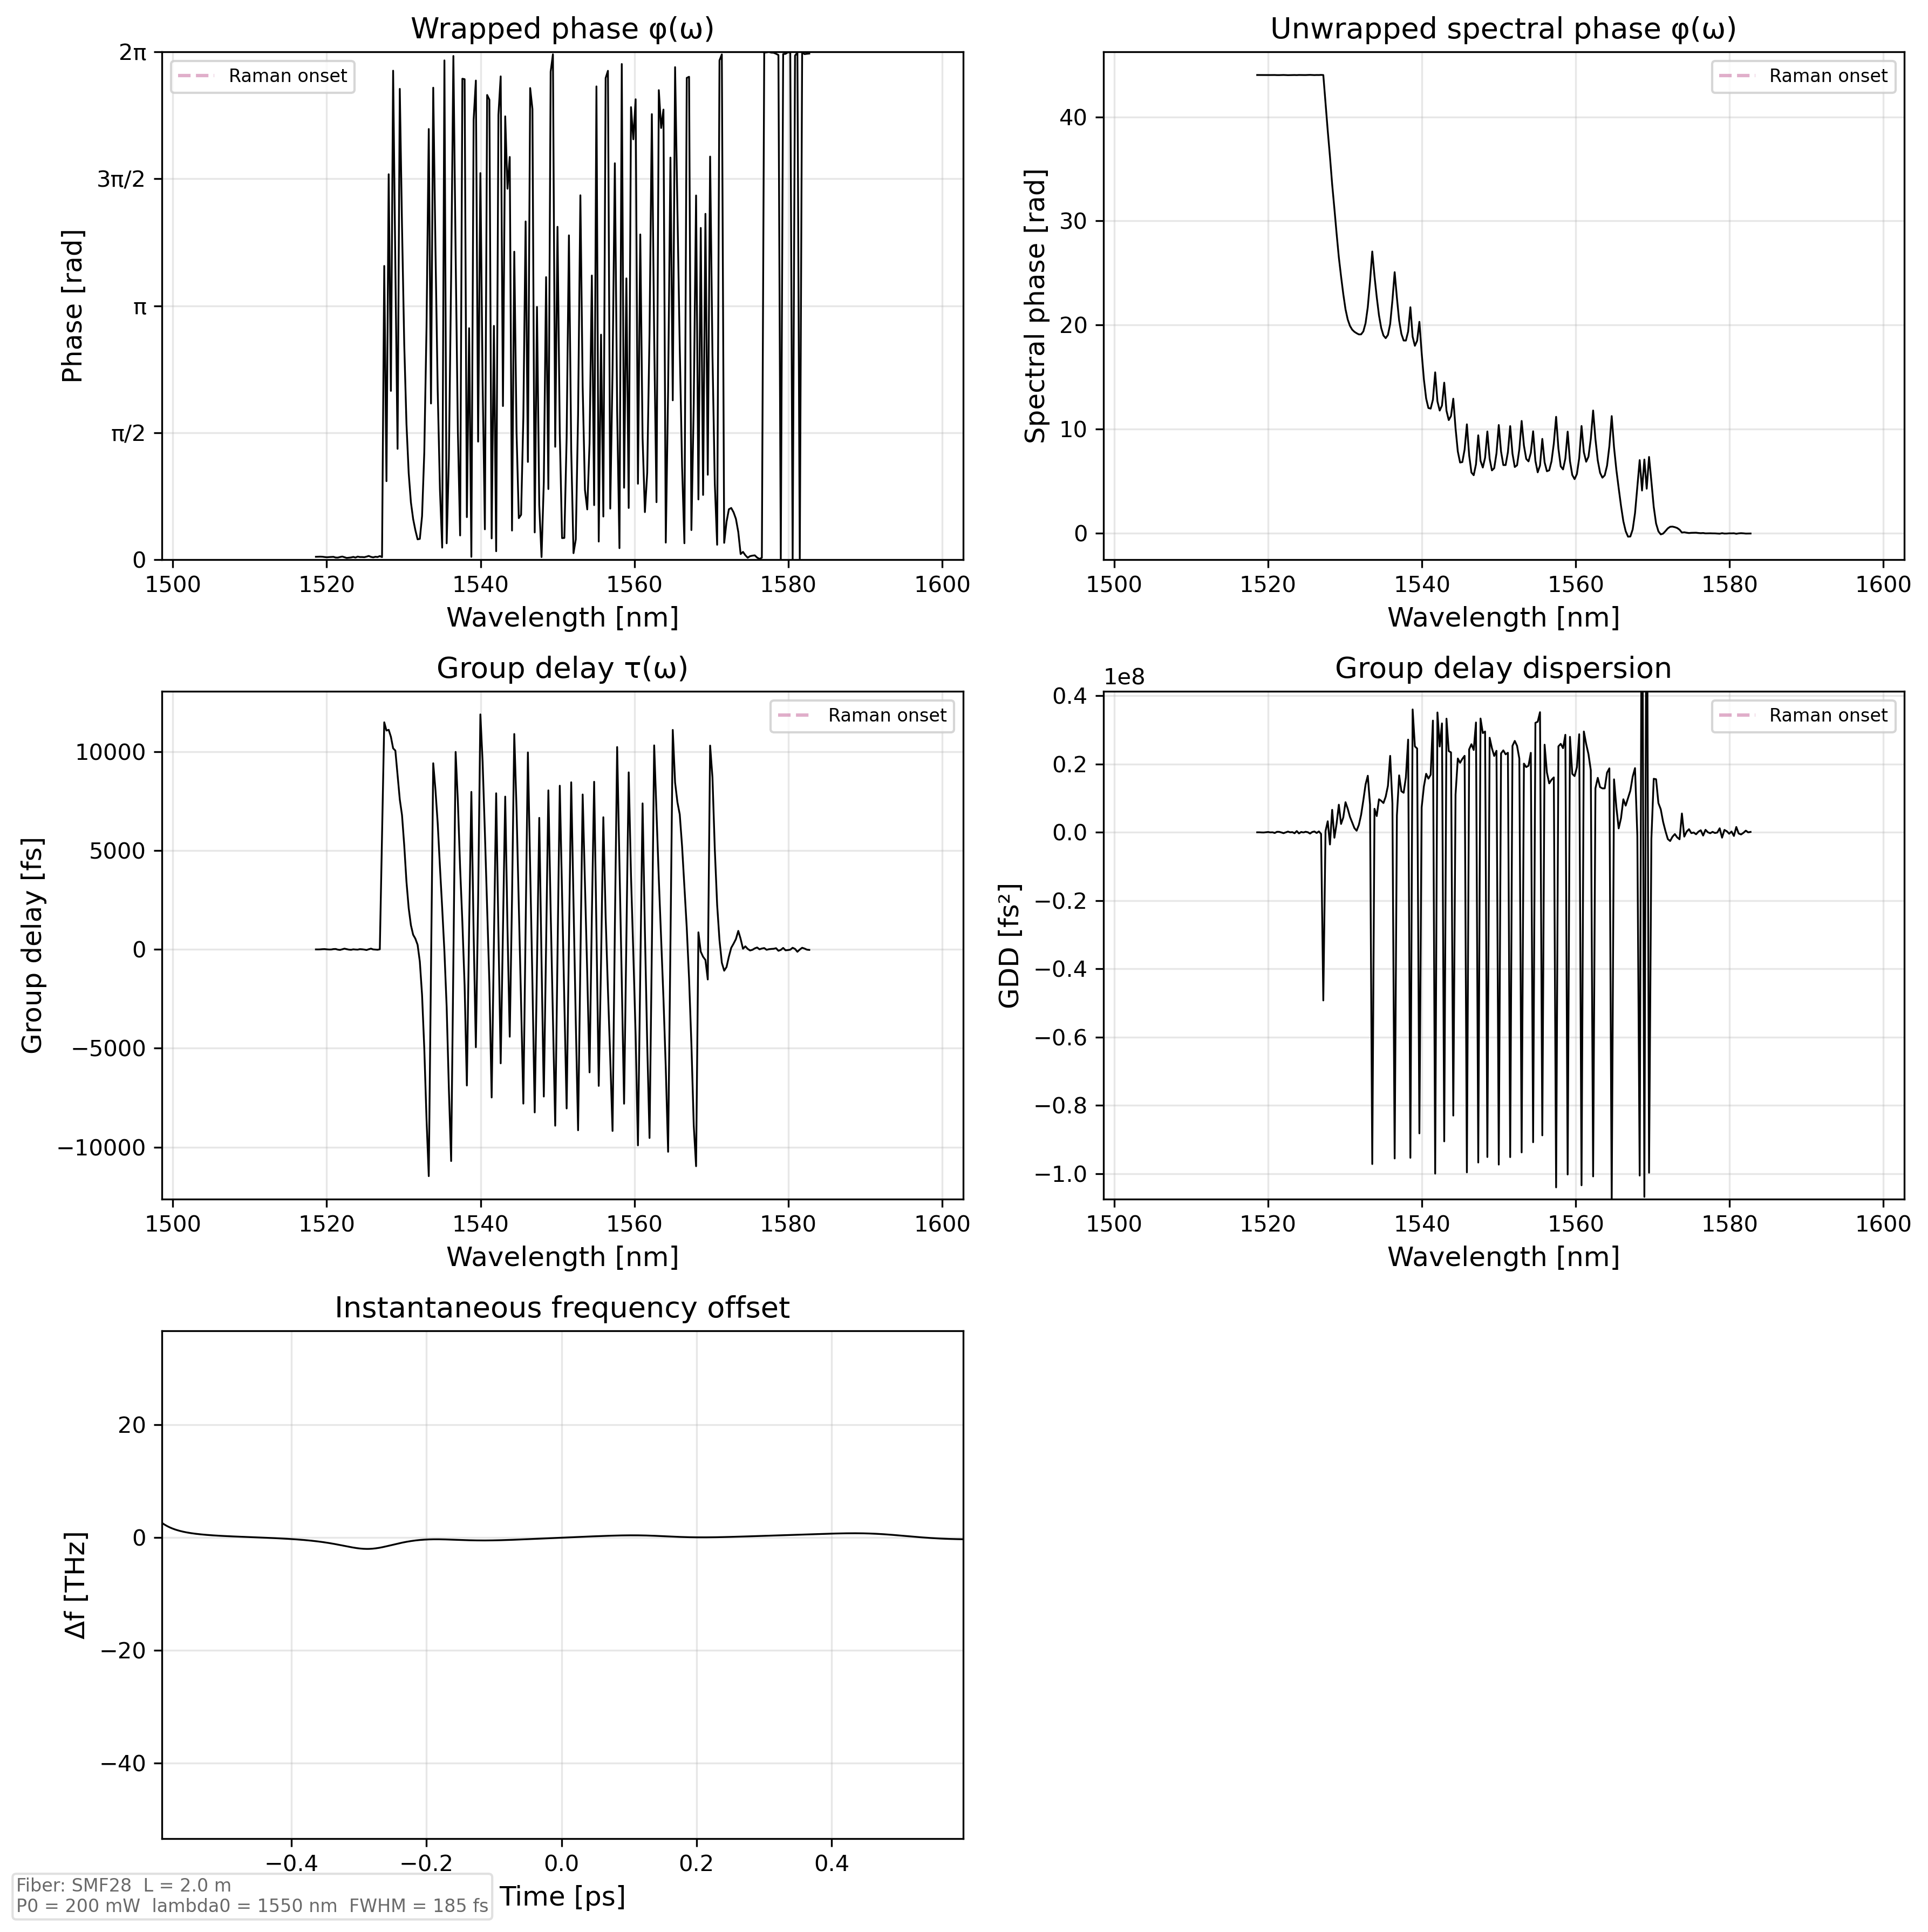
\includegraphics[height=0.47\textheight]{figures/cubic32_fullgrid_phase_diagnostic.png}
\vspace{0.5em}

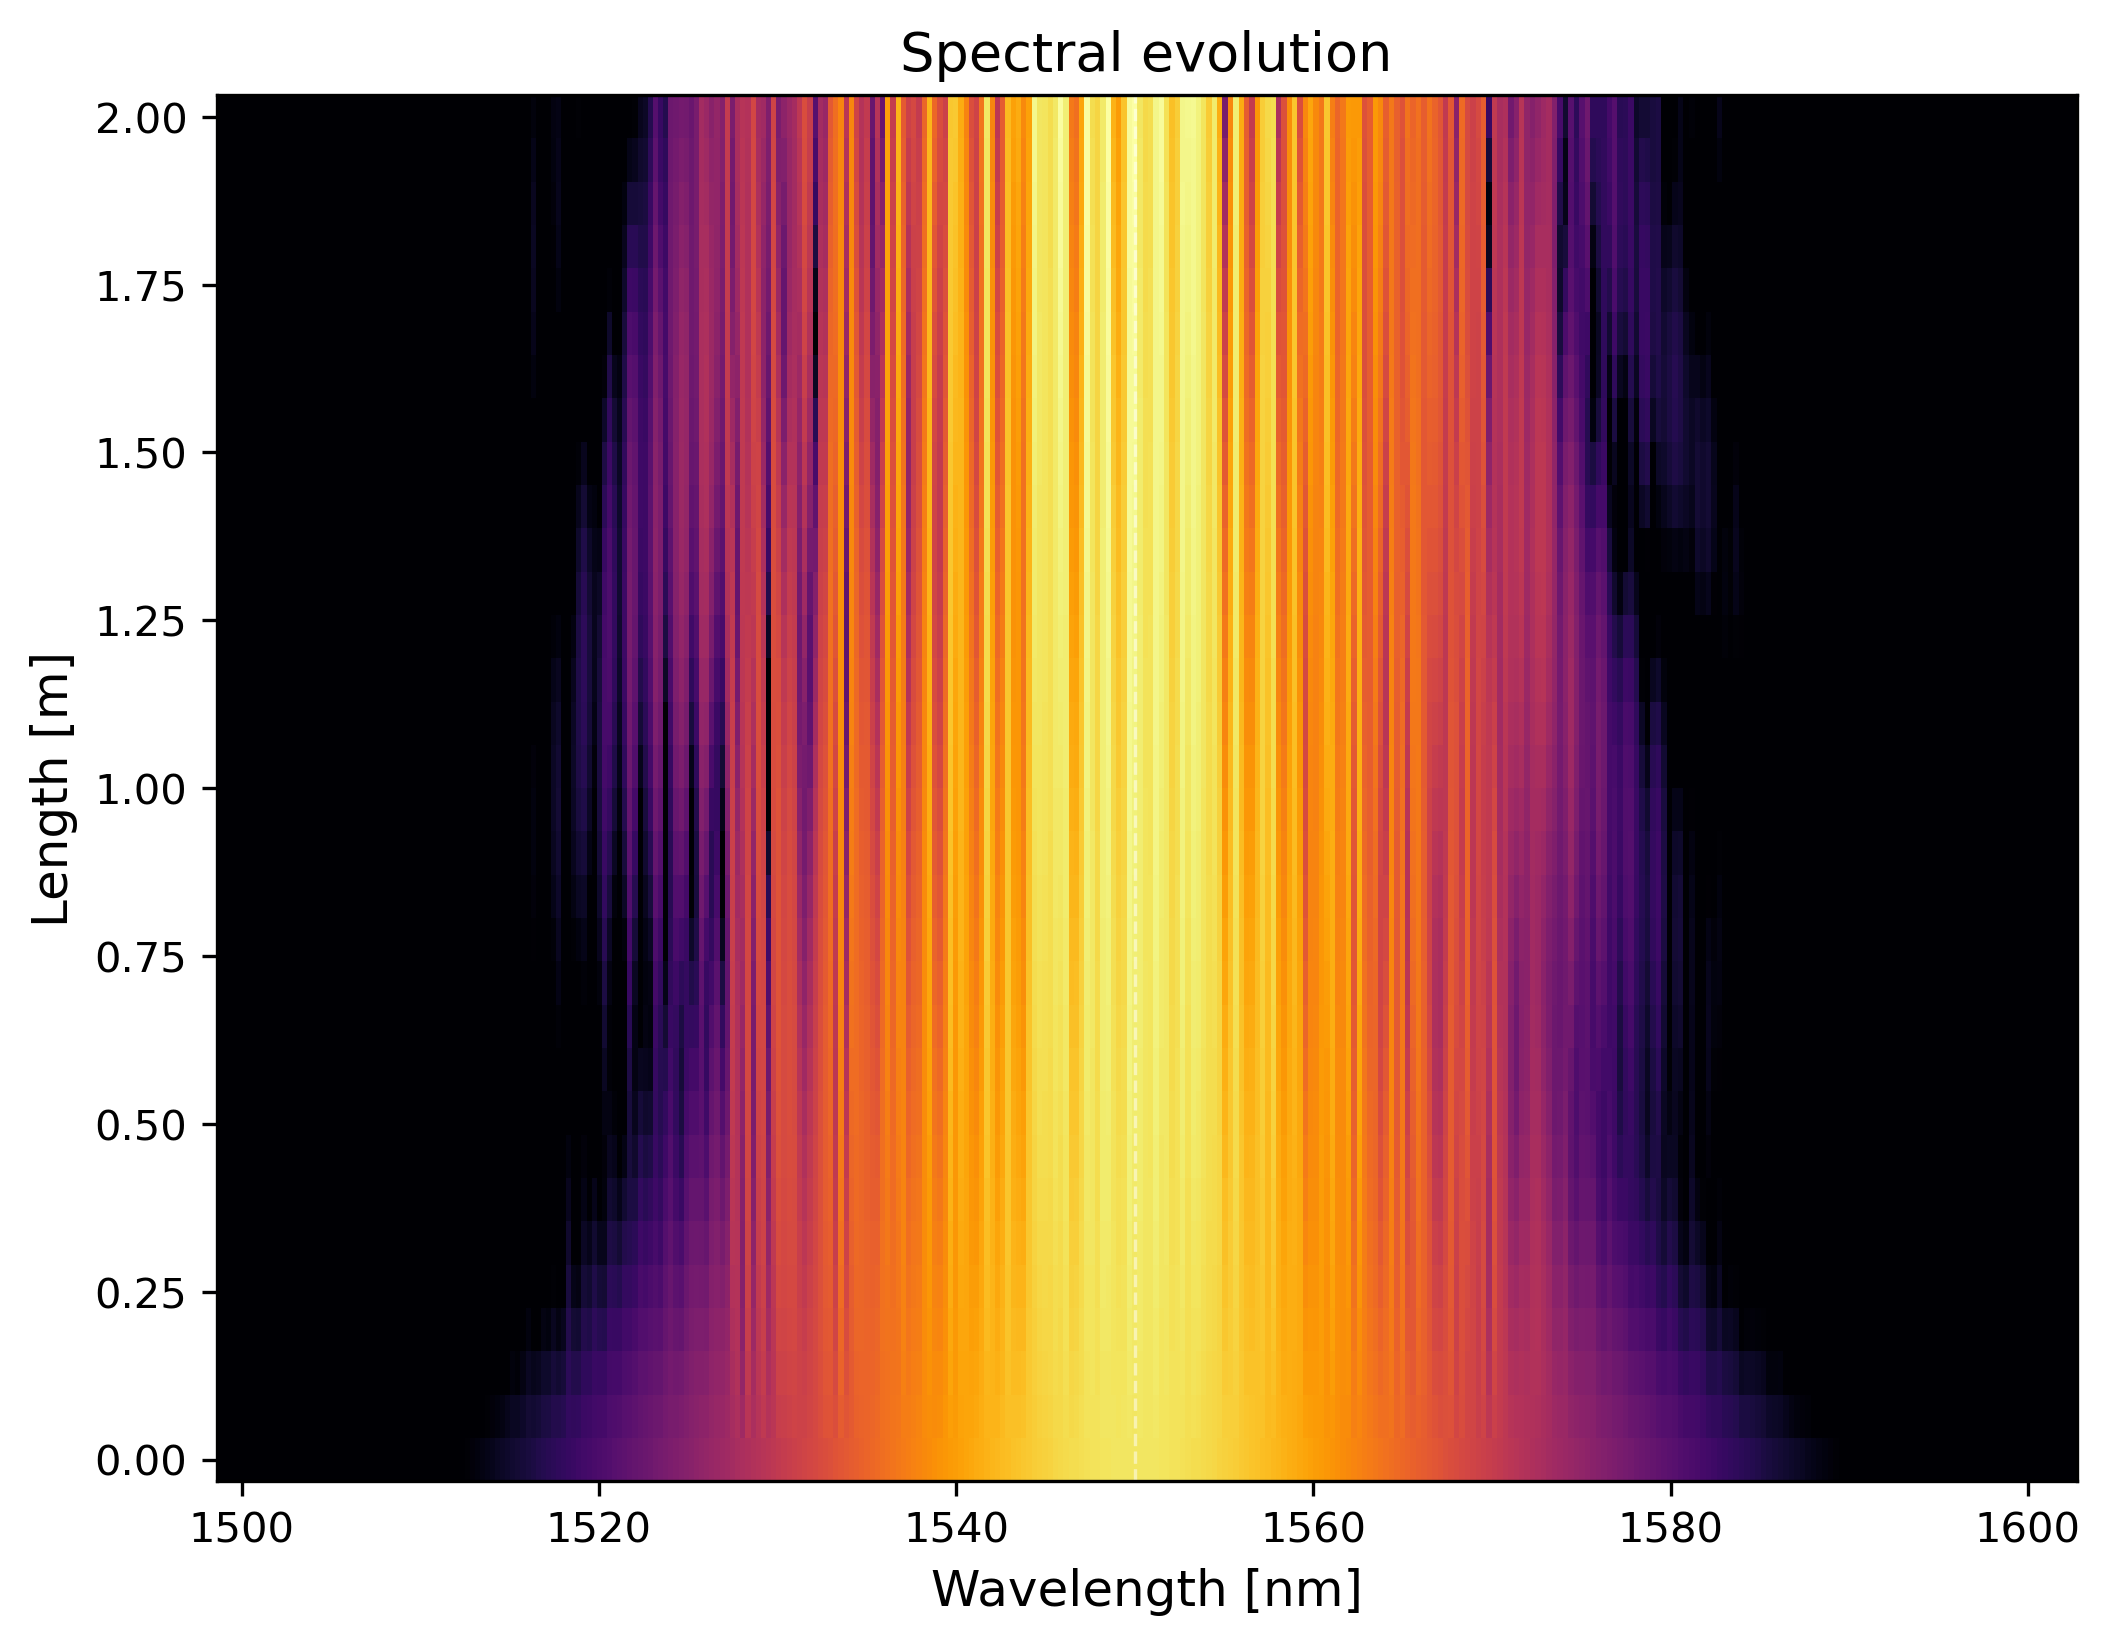
\includegraphics[height=0.31\textheight]{figures/cubic32_fullgrid_evolution.png}
\caption{Full-grid refinement from a cubic-continuation seed. The pair shows
that the seed survives the move into the full phase grid and ends up in the
deep canonical-specific family.}
\end{figure}

\clearpage
\section{Interpretation}

\textbf{The reduced basis is an access mechanism.} The main win is not merely
lower dimension. It is that the continuation path enters a solution family that
zero-start full-grid L-BFGS fails to reach.

\textbf{Local support matters.} Cubic splines strongly outperform global DCT
modes at comparable dimensionality. The useful phase structure is localized and
piecewise smooth, not simply globally smooth.

\textbf{Depth is not robustness.} The deepest cubic continuation solution has
\(\sigmathreedb \approx 0.07\,\mathrm{rad}\). Lower-dimensional or simpler
solutions are less suppressive but can tolerate larger perturbations.

\textbf{Depth is not transferability.} The polynomial profile is much shallower
but transfers across fiber choice with almost no penalty. The deep cubic family
is canonical-specific.

\section{Presentation Capsule}

If this note becomes a presentation block, the clean message is:
\begin{itemize}
    \item Reduced basis means \(\phi=Bc\): the optimizer moves a small coefficient vector, but the full-resolution fiber solver still evaluates the resulting phase.
    \item The reduced gradient is \(B^\top\nabla_\phi F\), which is just the chain rule for the map from coefficients to full-grid phase.
    \item The important result is basin access: the structured continuation path found deeper canonical solutions than zero-start full-grid L-BFGS.
    \item The limitation is just as important: the deepest profiles are narrow and fiber-specific, while simpler profiles are easier to transfer.
\end{itemize}

\section{Limitations}

The full ambient Hessian around the deepest reduced-basis optima has not been
fully mapped. The full-grid refinement test reduces the concern that the result
is a pure coordinate artifact, but it does not prove the deep basin is broad in
all \(16384\) spectral-phase directions.

The transfer result is currently asymmetric: transfer was evaluated from the
SMF-28-optimized profiles into HNLF and perturbed canonical settings. A symmetric
rerun optimized directly on HNLF would clarify whether the poor HNLF transfer is
a property of the basis family or of the canonical optimum.

The current note is based on completed local artifacts, not a single cleaned
reproduction command. A future methods pass should provide one public-facing
rerun recipe that reproduces the basis sweep, the penalty sweep, and the
full-grid refinement check.

\section{Operational Takeaway}

For canonical single-mode suppression, reduced-basis continuation is the best
known route into the deepest basin. For portable profile design, the simple
polynomial/quadratic-chirp family is the safer starting point. These are not the
same design objective, and future optimization reports should always show depth,
basin width, and transfer behavior together.

\section{Sources and References}

The external references below support the physics model, numerical propagation
method, optimizer choice, spline basis, and continuation idea. The numerical
values and figures in this note come from the project's archived reduced-basis,
penalty-sweep, transfer, and full-grid-refinement result artifacts.

\begin{thebibliography}{9}

\bibitem{agrawal2019}
G. P. Agrawal.
\textit{Nonlinear Fiber Optics}, 6th ed.
Academic Press, 2019.
\url{https://www.sciencedirect.com/book/9780128170427/nonlinear-fiber-optics}

\bibitem{dudley2006}
J. M. Dudley, G. Genty, and S. Coen.
``Supercontinuum generation in photonic crystal fiber.''
\textit{Reviews of Modern Physics}, 78, 1135--1184, 2006.
\url{https://doi.org/10.1103/RevModPhys.78.1135}

\bibitem{hult2007}
J. Hult.
``A fourth-order Runge-Kutta in the interaction picture method for simulating
supercontinuum generation in optical fibres.''
\textit{Journal of Lightwave Technology}, 25(12), 3770--3775, 2007.
\url{https://doi.org/10.1109/JLT.2007.909373}

\bibitem{liu1989}
D. C. Liu and J. Nocedal.
``On the limited memory BFGS method for large scale optimization.''
\textit{Mathematical Programming}, 45, 503--528, 1989.
\url{https://doi.org/10.1007/BF01589116}

\bibitem{nocedal2006}
J. Nocedal and S. J. Wright.
\textit{Numerical Optimization}, 2nd ed.
Springer, 2006.
\url{https://link.springer.com/book/10.1007/978-0-387-40065-5}

\bibitem{deboor2001}
C. de Boor.
\textit{A Practical Guide to Splines}, revised ed.
Springer, 2001.
\url{https://link.springer.com/book/9780387953663}

\bibitem{allgower1990}
E. L. Allgower and K. Georg.
\textit{Numerical Continuation Methods: An Introduction}.
Springer, 1990.
\url{https://link.springer.com/book/10.1007/978-3-642-61257-2}

\end{thebibliography}

\end{document}
